The \textit{total} partonic cross sections can be computed by
\begin{align}
\sigma^{(n)}_{k,j}(s,q^2,m^2) &= \int\limits_{-s'(1+\beta)/2}^{-s'(1-\beta)/2} dt_1\int\limits_0^{s_{4,max}}ds_4 \frac{d^2\sigma^{(n),fin}_{k,j}(s',t_1,u_1,q^2)}{dt_1ds_4}\\
s_{4,max} &= \frac{s}{s' t_1}\left(t_1+\frac{s'(1-\beta)}{2}\right)\left(t_1+\frac{s'(1+\beta)}{2}\right)
\end{align}
where $k$ denotes as usual projection, $j\in\{\Pg,\Pq,\Paq\}$ is a parton index and we used $s_4 = s'+t_1+u_1$. The result can then be parametrised as
\begin{align}
&\sigma_{k,j}(s,q^2,m^2)\nonumber\\
 &= \sigma^{(0)}_{k,j}(s,q^2,m^2) + \sigma^{(1)}_{k,j}(s,q^2,m^2)\\
 &= \frac{\alpha\alpha_S}{m^2}\left(f_{k,j}^{(0)}(\eta,\xi) + 4\pi\left(f_{k,j}^{(1)}(\eta,\xi) + \ln(\mu_F^2/m^2)\bar f_{k,j}^{F,(1)}(\eta,\xi) + \ln(\mu_R^2/m^2)\bar f_{k,j}^{R,(1)}(\eta,\xi)\right)\right)
\end{align}
where each function $f_{k,j}$ depends on the scaling variables $\eta=1/\rho-1$ and $\xi=-q^2/m^2$ and can be further decomposed by the electric charges
\begin{align}
f_{k,\Pg}(\eta,\xi) &= e_H^2 c_{k,\Pg}(\eta,\xi)\\
f_{k,\Pq}(\eta,\xi) &= e_H^2 c_{k,\Pq}(\eta,\xi) + e_L^2 d_{k,\Pq}(\eta,\xi)
\end{align}
As already mentioned the interference term proportional to $e_H e_L$ vanishes for total cross sections.

\fxerror{shift to appendix?}
\fxerror{compare T and P?}
\fxerror{how much to comment?}

\pagebreak
\begin{figure}[ht!]
\centering
\begin{subfigure}[t]{\textwidth}
	% GNUPLOT: LaTeX picture with Postscript
\begingroup
  \makeatletter
  \providecommand\color[2][]{%
    \GenericError{(gnuplot) \space\space\space\@spaces}{%
      Package color not loaded in conjunction with
      terminal option `colourtext'%
    }{See the gnuplot documentation for explanation.%
    }{Either use 'blacktext' in gnuplot or load the package
      color.sty in LaTeX.}%
    \renewcommand\color[2][]{}%
  }%
  \providecommand\includegraphics[2][]{%
    \GenericError{(gnuplot) \space\space\space\@spaces}{%
      Package graphicx or graphics not loaded%
    }{See the gnuplot documentation for explanation.%
    }{The gnuplot epslatex terminal needs graphicx.sty or graphics.sty.}%
    \renewcommand\includegraphics[2][]{}%
  }%
  \providecommand\rotatebox[2]{#2}%
  \@ifundefined{ifGPcolor}{%
    \newif\ifGPcolor
    \GPcolorfalse
  }{}%
  \@ifundefined{ifGPblacktext}{%
    \newif\ifGPblacktext
    \GPblacktexttrue
  }{}%
  % define a \g@addto@macro without @ in the name:
  \let\gplgaddtomacro\g@addto@macro
  % define empty templates for all commands taking text:
  \gdef\gplbacktext{}%
  \gdef\gplfronttext{}%
  \makeatother
  \ifGPblacktext
    % no textcolor at all
    \def\colorrgb#1{}%
    \def\colorgray#1{}%
  \else
    % gray or color?
    \ifGPcolor
      \def\colorrgb#1{\color[rgb]{#1}}%
      \def\colorgray#1{\color[gray]{#1}}%
      \expandafter\def\csname LTw\endcsname{\color{white}}%
      \expandafter\def\csname LTb\endcsname{\color{black}}%
      \expandafter\def\csname LTa\endcsname{\color{black}}%
      \expandafter\def\csname LT0\endcsname{\color[rgb]{1,0,0}}%
      \expandafter\def\csname LT1\endcsname{\color[rgb]{0,1,0}}%
      \expandafter\def\csname LT2\endcsname{\color[rgb]{0,0,1}}%
      \expandafter\def\csname LT3\endcsname{\color[rgb]{1,0,1}}%
      \expandafter\def\csname LT4\endcsname{\color[rgb]{0,1,1}}%
      \expandafter\def\csname LT5\endcsname{\color[rgb]{1,1,0}}%
      \expandafter\def\csname LT6\endcsname{\color[rgb]{0,0,0}}%
      \expandafter\def\csname LT7\endcsname{\color[rgb]{1,0.3,0}}%
      \expandafter\def\csname LT8\endcsname{\color[rgb]{0.5,0.5,0.5}}%
    \else
      % gray
      \def\colorrgb#1{\color{black}}%
      \def\colorgray#1{\color[gray]{#1}}%
      \expandafter\def\csname LTw\endcsname{\color{white}}%
      \expandafter\def\csname LTb\endcsname{\color{black}}%
      \expandafter\def\csname LTa\endcsname{\color{black}}%
      \expandafter\def\csname LT0\endcsname{\color{black}}%
      \expandafter\def\csname LT1\endcsname{\color{black}}%
      \expandafter\def\csname LT2\endcsname{\color{black}}%
      \expandafter\def\csname LT3\endcsname{\color{black}}%
      \expandafter\def\csname LT4\endcsname{\color{black}}%
      \expandafter\def\csname LT5\endcsname{\color{black}}%
      \expandafter\def\csname LT6\endcsname{\color{black}}%
      \expandafter\def\csname LT7\endcsname{\color{black}}%
      \expandafter\def\csname LT8\endcsname{\color{black}}%
    \fi
  \fi
    \setlength{\unitlength}{0.0500bp}%
    \ifx\gptboxheight\undefined%
      \newlength{\gptboxheight}%
      \newlength{\gptboxwidth}%
      \newsavebox{\gptboxtext}%
    \fi%
    \setlength{\fboxrule}{0.5pt}%
    \setlength{\fboxsep}{1pt}%
\begin{picture}(7920.00,4082.40)%
    \gplgaddtomacro\gplbacktext{%
      \csname LTb\endcsname%
      \put(726,220){\makebox(0,0)[r]{\strut{} 0.0}}%
      \put(726,820){\makebox(0,0)[r]{\strut{} 0.2}}%
      \put(726,1419){\makebox(0,0)[r]{\strut{} 0.4}}%
      \put(726,2019){\makebox(0,0)[r]{\strut{} 0.6}}%
      \put(726,2619){\makebox(0,0)[r]{\strut{} 0.8}}%
      \put(726,3218){\makebox(0,0)[r]{\strut{} 1.0}}%
      \put(726,3818){\makebox(0,0)[r]{\strut{} 1.2}}%
      \put(858,0){\makebox(0,0){\strut{}$0.001$}}%
      \put(1969,0){\makebox(0,0){\strut{}$0.01$}}%
      \put(3079,0){\makebox(0,0){\strut{}$0.1$}}%
      \put(4190,0){\makebox(0,0){\strut{}$1$}}%
      \put(5301,0){\makebox(0,0){\strut{}$10$}}%
      \put(6411,0){\makebox(0,0){\strut{}$100$}}%
      \put(7522,0){\makebox(0,0){\strut{}$1000$}}%
      \put(991,3458){\makebox(0,0)[l]{\strut{}(a) $c_{T,g}^{(0)}(\eta)$}}%
    }%
    \gplgaddtomacro\gplfronttext{%
      \csname LTb\endcsname%
      \put(5611,3645){\makebox(0,0)[l]{\strut{}$Q^2=10^{-2}$}}%
      \csname LTb\endcsname%
      \put(5611,3425){\makebox(0,0)[l]{\strut{}$Q^2=10^0$}}%
      \csname LTb\endcsname%
      \put(5611,3205){\makebox(0,0)[l]{\strut{}$Q^2=10^1$}}%
      \csname LTb\endcsname%
      \put(5611,2985){\makebox(0,0)[l]{\strut{}$Q^2=10^2$}}%
      \csname LTb\endcsname%
      \put(5611,2765){\makebox(0,0)[l]{\strut{}$Q^2=10^3$}}%
    }%
    \gplbacktext
    \put(0,0){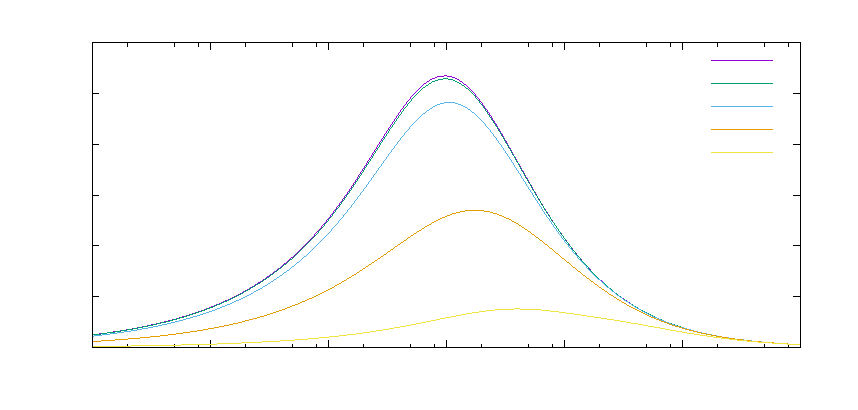
\includegraphics{img/cg0T}}%
    \gplfronttext
  \end{picture}%
\endgroup

\end{subfigure}\\%
\begin{subfigure}[t]{\textwidth}
	% GNUPLOT: LaTeX picture with Postscript
\begingroup
  \makeatletter
  \providecommand\color[2][]{%
    \GenericError{(gnuplot) \space\space\space\@spaces}{%
      Package color not loaded in conjunction with
      terminal option `colourtext'%
    }{See the gnuplot documentation for explanation.%
    }{Either use 'blacktext' in gnuplot or load the package
      color.sty in LaTeX.}%
    \renewcommand\color[2][]{}%
  }%
  \providecommand\includegraphics[2][]{%
    \GenericError{(gnuplot) \space\space\space\@spaces}{%
      Package graphicx or graphics not loaded%
    }{See the gnuplot documentation for explanation.%
    }{The gnuplot epslatex terminal needs graphicx.sty or graphics.sty.}%
    \renewcommand\includegraphics[2][]{}%
  }%
  \providecommand\rotatebox[2]{#2}%
  \@ifundefined{ifGPcolor}{%
    \newif\ifGPcolor
    \GPcolorfalse
  }{}%
  \@ifundefined{ifGPblacktext}{%
    \newif\ifGPblacktext
    \GPblacktexttrue
  }{}%
  % define a \g@addto@macro without @ in the name:
  \let\gplgaddtomacro\g@addto@macro
  % define empty templates for all commands taking text:
  \gdef\gplbacktext{}%
  \gdef\gplfronttext{}%
  \makeatother
  \ifGPblacktext
    % no textcolor at all
    \def\colorrgb#1{}%
    \def\colorgray#1{}%
  \else
    % gray or color?
    \ifGPcolor
      \def\colorrgb#1{\color[rgb]{#1}}%
      \def\colorgray#1{\color[gray]{#1}}%
      \expandafter\def\csname LTw\endcsname{\color{white}}%
      \expandafter\def\csname LTb\endcsname{\color{black}}%
      \expandafter\def\csname LTa\endcsname{\color{black}}%
      \expandafter\def\csname LT0\endcsname{\color[rgb]{1,0,0}}%
      \expandafter\def\csname LT1\endcsname{\color[rgb]{0,1,0}}%
      \expandafter\def\csname LT2\endcsname{\color[rgb]{0,0,1}}%
      \expandafter\def\csname LT3\endcsname{\color[rgb]{1,0,1}}%
      \expandafter\def\csname LT4\endcsname{\color[rgb]{0,1,1}}%
      \expandafter\def\csname LT5\endcsname{\color[rgb]{1,1,0}}%
      \expandafter\def\csname LT6\endcsname{\color[rgb]{0,0,0}}%
      \expandafter\def\csname LT7\endcsname{\color[rgb]{1,0.3,0}}%
      \expandafter\def\csname LT8\endcsname{\color[rgb]{0.5,0.5,0.5}}%
    \else
      % gray
      \def\colorrgb#1{\color{black}}%
      \def\colorgray#1{\color[gray]{#1}}%
      \expandafter\def\csname LTw\endcsname{\color{white}}%
      \expandafter\def\csname LTb\endcsname{\color{black}}%
      \expandafter\def\csname LTa\endcsname{\color{black}}%
      \expandafter\def\csname LT0\endcsname{\color{black}}%
      \expandafter\def\csname LT1\endcsname{\color{black}}%
      \expandafter\def\csname LT2\endcsname{\color{black}}%
      \expandafter\def\csname LT3\endcsname{\color{black}}%
      \expandafter\def\csname LT4\endcsname{\color{black}}%
      \expandafter\def\csname LT5\endcsname{\color{black}}%
      \expandafter\def\csname LT6\endcsname{\color{black}}%
      \expandafter\def\csname LT7\endcsname{\color{black}}%
      \expandafter\def\csname LT8\endcsname{\color{black}}%
    \fi
  \fi
    \setlength{\unitlength}{0.0500bp}%
    \ifx\gptboxheight\undefined%
      \newlength{\gptboxheight}%
      \newlength{\gptboxwidth}%
      \newsavebox{\gptboxtext}%
    \fi%
    \setlength{\fboxrule}{0.5pt}%
    \setlength{\fboxsep}{1pt}%
\begin{picture}(7920.00,4082.40)%
    \gplgaddtomacro\gplbacktext{%
      \csname LTb\endcsname%
      \put(726,220){\makebox(0,0)[r]{\strut{}0.00}}%
      \put(726,734){\makebox(0,0)[r]{\strut{}0.02}}%
      \put(726,1248){\makebox(0,0)[r]{\strut{}0.04}}%
      \put(726,1762){\makebox(0,0)[r]{\strut{}0.06}}%
      \put(726,2276){\makebox(0,0)[r]{\strut{}0.08}}%
      \put(726,2790){\makebox(0,0)[r]{\strut{}0.10}}%
      \put(726,3304){\makebox(0,0)[r]{\strut{}0.12}}%
      \put(726,3818){\makebox(0,0)[r]{\strut{}0.14}}%
      \put(858,0){\makebox(0,0){\strut{}$0.001$}}%
      \put(1969,0){\makebox(0,0){\strut{}$0.01$}}%
      \put(3079,0){\makebox(0,0){\strut{}$0.1$}}%
      \put(4190,0){\makebox(0,0){\strut{}$1$}}%
      \put(5301,0){\makebox(0,0){\strut{}$10$}}%
      \put(6411,0){\makebox(0,0){\strut{}$100$}}%
      \put(7522,0){\makebox(0,0){\strut{}$1000$}}%
      \put(991,3458){\makebox(0,0)[l]{\strut{}(b) $c_{L,g}^{(0)}(\eta)$}}%
    }%
    \gplgaddtomacro\gplfronttext{%
      \csname LTb\endcsname%
      \put(5611,3645){\makebox(0,0)[l]{\strut{}$Q^2=10^{-2}$}}%
      \csname LTb\endcsname%
      \put(5611,3425){\makebox(0,0)[l]{\strut{}$Q^2=10^0$}}%
      \csname LTb\endcsname%
      \put(5611,3205){\makebox(0,0)[l]{\strut{}$Q^2=10^1$}}%
      \csname LTb\endcsname%
      \put(5611,2985){\makebox(0,0)[l]{\strut{}$Q^2=10^2$}}%
      \csname LTb\endcsname%
      \put(5611,2765){\makebox(0,0)[l]{\strut{}$Q^2=10^3$}}%
    }%
    \gplbacktext
    \put(0,0){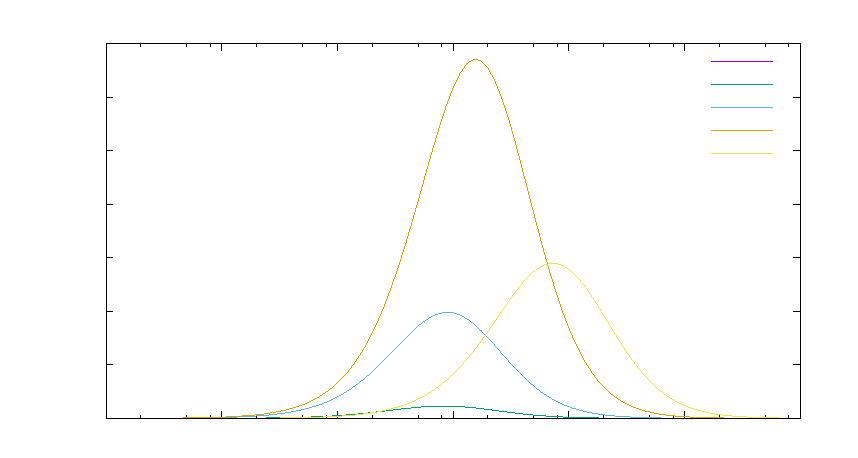
\includegraphics{img/cg0L}}%
    \gplfronttext
  \end{picture}%
\endgroup

\end{subfigure}\\%
\begin{subfigure}[t]{\textwidth}
	% GNUPLOT: LaTeX picture with Postscript
\begingroup
  \makeatletter
  \providecommand\color[2][]{%
    \GenericError{(gnuplot) \space\space\space\@spaces}{%
      Package color not loaded in conjunction with
      terminal option `colourtext'%
    }{See the gnuplot documentation for explanation.%
    }{Either use 'blacktext' in gnuplot or load the package
      color.sty in LaTeX.}%
    \renewcommand\color[2][]{}%
  }%
  \providecommand\includegraphics[2][]{%
    \GenericError{(gnuplot) \space\space\space\@spaces}{%
      Package graphicx or graphics not loaded%
    }{See the gnuplot documentation for explanation.%
    }{The gnuplot epslatex terminal needs graphicx.sty or graphics.sty.}%
    \renewcommand\includegraphics[2][]{}%
  }%
  \providecommand\rotatebox[2]{#2}%
  \@ifundefined{ifGPcolor}{%
    \newif\ifGPcolor
    \GPcolorfalse
  }{}%
  \@ifundefined{ifGPblacktext}{%
    \newif\ifGPblacktext
    \GPblacktexttrue
  }{}%
  % define a \g@addto@macro without @ in the name:
  \let\gplgaddtomacro\g@addto@macro
  % define empty templates for all commands taking text:
  \gdef\gplbacktext{}%
  \gdef\gplfronttext{}%
  \makeatother
  \ifGPblacktext
    % no textcolor at all
    \def\colorrgb#1{}%
    \def\colorgray#1{}%
  \else
    % gray or color?
    \ifGPcolor
      \def\colorrgb#1{\color[rgb]{#1}}%
      \def\colorgray#1{\color[gray]{#1}}%
      \expandafter\def\csname LTw\endcsname{\color{white}}%
      \expandafter\def\csname LTb\endcsname{\color{black}}%
      \expandafter\def\csname LTa\endcsname{\color{black}}%
      \expandafter\def\csname LT0\endcsname{\color[rgb]{1,0,0}}%
      \expandafter\def\csname LT1\endcsname{\color[rgb]{0,1,0}}%
      \expandafter\def\csname LT2\endcsname{\color[rgb]{0,0,1}}%
      \expandafter\def\csname LT3\endcsname{\color[rgb]{1,0,1}}%
      \expandafter\def\csname LT4\endcsname{\color[rgb]{0,1,1}}%
      \expandafter\def\csname LT5\endcsname{\color[rgb]{1,1,0}}%
      \expandafter\def\csname LT6\endcsname{\color[rgb]{0,0,0}}%
      \expandafter\def\csname LT7\endcsname{\color[rgb]{1,0.3,0}}%
      \expandafter\def\csname LT8\endcsname{\color[rgb]{0.5,0.5,0.5}}%
    \else
      % gray
      \def\colorrgb#1{\color{black}}%
      \def\colorgray#1{\color[gray]{#1}}%
      \expandafter\def\csname LTw\endcsname{\color{white}}%
      \expandafter\def\csname LTb\endcsname{\color{black}}%
      \expandafter\def\csname LTa\endcsname{\color{black}}%
      \expandafter\def\csname LT0\endcsname{\color{black}}%
      \expandafter\def\csname LT1\endcsname{\color{black}}%
      \expandafter\def\csname LT2\endcsname{\color{black}}%
      \expandafter\def\csname LT3\endcsname{\color{black}}%
      \expandafter\def\csname LT4\endcsname{\color{black}}%
      \expandafter\def\csname LT5\endcsname{\color{black}}%
      \expandafter\def\csname LT6\endcsname{\color{black}}%
      \expandafter\def\csname LT7\endcsname{\color{black}}%
      \expandafter\def\csname LT8\endcsname{\color{black}}%
    \fi
  \fi
    \setlength{\unitlength}{0.0500bp}%
    \ifx\gptboxheight\undefined%
      \newlength{\gptboxheight}%
      \newlength{\gptboxwidth}%
      \newsavebox{\gptboxtext}%
    \fi%
    \setlength{\fboxrule}{0.5pt}%
    \setlength{\fboxsep}{1pt}%
\begin{picture}(7920.00,4082.40)%
    \gplgaddtomacro\gplbacktext{%
      \csname LTb\endcsname%
      \put(726,220){\makebox(0,0)[r]{\strut{}-0.2}}%
      \put(726,734){\makebox(0,0)[r]{\strut{}-0.1}}%
      \put(726,1248){\makebox(0,0)[r]{\strut{}0.0}}%
      \put(726,1762){\makebox(0,0)[r]{\strut{}0.1}}%
      \put(726,2276){\makebox(0,0)[r]{\strut{}0.2}}%
      \put(726,2790){\makebox(0,0)[r]{\strut{}0.3}}%
      \put(726,3304){\makebox(0,0)[r]{\strut{}0.4}}%
      \put(726,3818){\makebox(0,0)[r]{\strut{}0.5}}%
      \put(858,0){\makebox(0,0){\strut{}$0.001$}}%
      \put(1969,0){\makebox(0,0){\strut{}$0.01$}}%
      \put(3079,0){\makebox(0,0){\strut{}$0.1$}}%
      \put(4190,0){\makebox(0,0){\strut{}$1$}}%
      \put(5301,0){\makebox(0,0){\strut{}$10$}}%
      \put(6411,0){\makebox(0,0){\strut{}$100$}}%
      \put(7522,0){\makebox(0,0){\strut{}$1000$}}%
      \put(991,3458){\makebox(0,0)[l]{\strut{}(c) $c_{P,g}^{(0)}(\eta)$}}%
    }%
    \gplgaddtomacro\gplfronttext{%
      \csname LTb\endcsname%
      \put(5611,3645){\makebox(0,0)[l]{\strut{}$Q^2=10^{-2}$}}%
      \csname LTb\endcsname%
      \put(5611,3425){\makebox(0,0)[l]{\strut{}$Q^2=10^0$}}%
      \csname LTb\endcsname%
      \put(5611,3205){\makebox(0,0)[l]{\strut{}$Q^2=10^1$}}%
      \csname LTb\endcsname%
      \put(5611,2985){\makebox(0,0)[l]{\strut{}$Q^2=10^2$}}%
      \csname LTb\endcsname%
      \put(5611,2765){\makebox(0,0)[l]{\strut{}$Q^2=10^3$}}%
    }%
    \gplbacktext
    \put(0,0){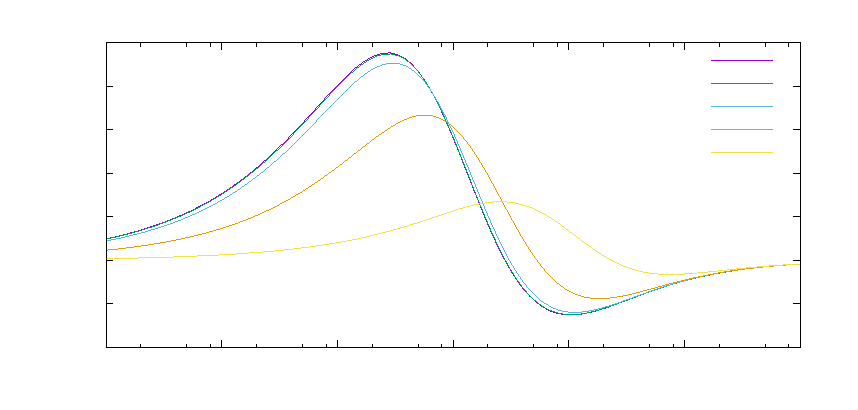
\includegraphics{img/cg0P}}%
    \gplfronttext
  \end{picture}%
\endgroup

\end{subfigure}
\caption{leading order scaling functions $c_{k,g}^{(0)}(\eta,\xi)$ plotted as function of $\eta=s/(4m^2)-1$ for different values of $Q^2$ in units of $\si{\GeV^2}$ at $m=\SI{4.75}{\GeV}$ (i.e. different values of $\xi=Q^2/m^2$) }\label{fig:cg0}
\end{figure}

\pagebreak
\begin{figure}[ht!]
\centering
\begin{subfigure}[t]{\textwidth}
	% GNUPLOT: LaTeX picture with Postscript
\begingroup
  \makeatletter
  \providecommand\color[2][]{%
    \GenericError{(gnuplot) \space\space\space\@spaces}{%
      Package color not loaded in conjunction with
      terminal option `colourtext'%
    }{See the gnuplot documentation for explanation.%
    }{Either use 'blacktext' in gnuplot or load the package
      color.sty in LaTeX.}%
    \renewcommand\color[2][]{}%
  }%
  \providecommand\includegraphics[2][]{%
    \GenericError{(gnuplot) \space\space\space\@spaces}{%
      Package graphicx or graphics not loaded%
    }{See the gnuplot documentation for explanation.%
    }{The gnuplot epslatex terminal needs graphicx.sty or graphics.sty.}%
    \renewcommand\includegraphics[2][]{}%
  }%
  \providecommand\rotatebox[2]{#2}%
  \@ifundefined{ifGPcolor}{%
    \newif\ifGPcolor
    \GPcolorfalse
  }{}%
  \@ifundefined{ifGPblacktext}{%
    \newif\ifGPblacktext
    \GPblacktexttrue
  }{}%
  % define a \g@addto@macro without @ in the name:
  \let\gplgaddtomacro\g@addto@macro
  % define empty templates for all commands taking text:
  \gdef\gplbacktext{}%
  \gdef\gplfronttext{}%
  \makeatother
  \ifGPblacktext
    % no textcolor at all
    \def\colorrgb#1{}%
    \def\colorgray#1{}%
  \else
    % gray or color?
    \ifGPcolor
      \def\colorrgb#1{\color[rgb]{#1}}%
      \def\colorgray#1{\color[gray]{#1}}%
      \expandafter\def\csname LTw\endcsname{\color{white}}%
      \expandafter\def\csname LTb\endcsname{\color{black}}%
      \expandafter\def\csname LTa\endcsname{\color{black}}%
      \expandafter\def\csname LT0\endcsname{\color[rgb]{1,0,0}}%
      \expandafter\def\csname LT1\endcsname{\color[rgb]{0,1,0}}%
      \expandafter\def\csname LT2\endcsname{\color[rgb]{0,0,1}}%
      \expandafter\def\csname LT3\endcsname{\color[rgb]{1,0,1}}%
      \expandafter\def\csname LT4\endcsname{\color[rgb]{0,1,1}}%
      \expandafter\def\csname LT5\endcsname{\color[rgb]{1,1,0}}%
      \expandafter\def\csname LT6\endcsname{\color[rgb]{0,0,0}}%
      \expandafter\def\csname LT7\endcsname{\color[rgb]{1,0.3,0}}%
      \expandafter\def\csname LT8\endcsname{\color[rgb]{0.5,0.5,0.5}}%
    \else
      % gray
      \def\colorrgb#1{\color{black}}%
      \def\colorgray#1{\color[gray]{#1}}%
      \expandafter\def\csname LTw\endcsname{\color{white}}%
      \expandafter\def\csname LTb\endcsname{\color{black}}%
      \expandafter\def\csname LTa\endcsname{\color{black}}%
      \expandafter\def\csname LT0\endcsname{\color{black}}%
      \expandafter\def\csname LT1\endcsname{\color{black}}%
      \expandafter\def\csname LT2\endcsname{\color{black}}%
      \expandafter\def\csname LT3\endcsname{\color{black}}%
      \expandafter\def\csname LT4\endcsname{\color{black}}%
      \expandafter\def\csname LT5\endcsname{\color{black}}%
      \expandafter\def\csname LT6\endcsname{\color{black}}%
      \expandafter\def\csname LT7\endcsname{\color{black}}%
      \expandafter\def\csname LT8\endcsname{\color{black}}%
    \fi
  \fi
    \setlength{\unitlength}{0.0500bp}%
    \ifx\gptboxheight\undefined%
      \newlength{\gptboxheight}%
      \newlength{\gptboxwidth}%
      \newsavebox{\gptboxtext}%
    \fi%
    \setlength{\fboxrule}{0.5pt}%
    \setlength{\fboxsep}{1pt}%
\begin{picture}(7920.00,3628.80)%
    \gplgaddtomacro\gplbacktext{%
      \csname LTb\endcsname%
      \put(726,440){\makebox(0,0)[r]{\strut{}-0.1}}%
      \put(726,806){\makebox(0,0)[r]{\strut{}0.0}}%
      \put(726,1171){\makebox(0,0)[r]{\strut{}0.1}}%
      \put(726,1537){\makebox(0,0)[r]{\strut{}0.1}}%
      \put(726,1902){\makebox(0,0)[r]{\strut{}0.2}}%
      \put(726,2268){\makebox(0,0)[r]{\strut{}0.2}}%
      \put(726,2633){\makebox(0,0)[r]{\strut{}0.2}}%
      \put(726,2999){\makebox(0,0)[r]{\strut{}0.3}}%
      \put(726,3364){\makebox(0,0)[r]{\strut{}0.3}}%
      \put(858,220){\makebox(0,0){\strut{}$0.001$}}%
      \put(1969,220){\makebox(0,0){\strut{}$0.01$}}%
      \put(3079,220){\makebox(0,0){\strut{}$0.1$}}%
      \put(4190,220){\makebox(0,0){\strut{}$1$}}%
      \put(5301,220){\makebox(0,0){\strut{}$10$}}%
      \put(6411,220){\makebox(0,0){\strut{}$100$}}%
      \put(7522,220){\makebox(0,0){\strut{}$1000$}}%
    }%
    \gplgaddtomacro\gplfronttext{%
      \csname LTb\endcsname%
      \put(4077,3108){\makebox(0,0)[l]{\strut{}$Q^2=10^{-2}$}}%
      \csname LTb\endcsname%
      \put(4077,2888){\makebox(0,0)[l]{\strut{}$Q^2=10^0$}}%
      \csname LTb\endcsname%
      \put(4077,2668){\makebox(0,0)[l]{\strut{}$Q^2=10^1$}}%
      \csname LTb\endcsname%
      \put(4077,2448){\makebox(0,0)[l]{\strut{}$Q^2=10^2$}}%
      \csname LTb\endcsname%
      \put(4077,2228){\makebox(0,0)[l]{\strut{}$Q^2=10^3$}}%
    }%
    \gplbacktext
    \put(0,0){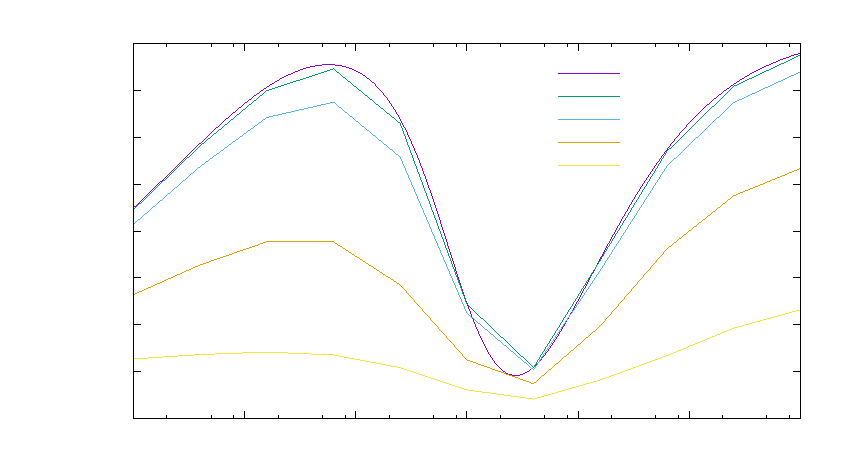
\includegraphics{img/cg1T}}%
    \gplfronttext
  \end{picture}%
\endgroup

\end{subfigure}\\%
\begin{subfigure}[t]{\textwidth}
	% GNUPLOT: LaTeX picture with Postscript
\begingroup
  \makeatletter
  \providecommand\color[2][]{%
    \GenericError{(gnuplot) \space\space\space\@spaces}{%
      Package color not loaded in conjunction with
      terminal option `colourtext'%
    }{See the gnuplot documentation for explanation.%
    }{Either use 'blacktext' in gnuplot or load the package
      color.sty in LaTeX.}%
    \renewcommand\color[2][]{}%
  }%
  \providecommand\includegraphics[2][]{%
    \GenericError{(gnuplot) \space\space\space\@spaces}{%
      Package graphicx or graphics not loaded%
    }{See the gnuplot documentation for explanation.%
    }{The gnuplot epslatex terminal needs graphicx.sty or graphics.sty.}%
    \renewcommand\includegraphics[2][]{}%
  }%
  \providecommand\rotatebox[2]{#2}%
  \@ifundefined{ifGPcolor}{%
    \newif\ifGPcolor
    \GPcolorfalse
  }{}%
  \@ifundefined{ifGPblacktext}{%
    \newif\ifGPblacktext
    \GPblacktexttrue
  }{}%
  % define a \g@addto@macro without @ in the name:
  \let\gplgaddtomacro\g@addto@macro
  % define empty templates for all commands taking text:
  \gdef\gplbacktext{}%
  \gdef\gplfronttext{}%
  \makeatother
  \ifGPblacktext
    % no textcolor at all
    \def\colorrgb#1{}%
    \def\colorgray#1{}%
  \else
    % gray or color?
    \ifGPcolor
      \def\colorrgb#1{\color[rgb]{#1}}%
      \def\colorgray#1{\color[gray]{#1}}%
      \expandafter\def\csname LTw\endcsname{\color{white}}%
      \expandafter\def\csname LTb\endcsname{\color{black}}%
      \expandafter\def\csname LTa\endcsname{\color{black}}%
      \expandafter\def\csname LT0\endcsname{\color[rgb]{1,0,0}}%
      \expandafter\def\csname LT1\endcsname{\color[rgb]{0,1,0}}%
      \expandafter\def\csname LT2\endcsname{\color[rgb]{0,0,1}}%
      \expandafter\def\csname LT3\endcsname{\color[rgb]{1,0,1}}%
      \expandafter\def\csname LT4\endcsname{\color[rgb]{0,1,1}}%
      \expandafter\def\csname LT5\endcsname{\color[rgb]{1,1,0}}%
      \expandafter\def\csname LT6\endcsname{\color[rgb]{0,0,0}}%
      \expandafter\def\csname LT7\endcsname{\color[rgb]{1,0.3,0}}%
      \expandafter\def\csname LT8\endcsname{\color[rgb]{0.5,0.5,0.5}}%
    \else
      % gray
      \def\colorrgb#1{\color{black}}%
      \def\colorgray#1{\color[gray]{#1}}%
      \expandafter\def\csname LTw\endcsname{\color{white}}%
      \expandafter\def\csname LTb\endcsname{\color{black}}%
      \expandafter\def\csname LTa\endcsname{\color{black}}%
      \expandafter\def\csname LT0\endcsname{\color{black}}%
      \expandafter\def\csname LT1\endcsname{\color{black}}%
      \expandafter\def\csname LT2\endcsname{\color{black}}%
      \expandafter\def\csname LT3\endcsname{\color{black}}%
      \expandafter\def\csname LT4\endcsname{\color{black}}%
      \expandafter\def\csname LT5\endcsname{\color{black}}%
      \expandafter\def\csname LT6\endcsname{\color{black}}%
      \expandafter\def\csname LT7\endcsname{\color{black}}%
      \expandafter\def\csname LT8\endcsname{\color{black}}%
    \fi
  \fi
    \setlength{\unitlength}{0.0500bp}%
    \ifx\gptboxheight\undefined%
      \newlength{\gptboxheight}%
      \newlength{\gptboxwidth}%
      \newsavebox{\gptboxtext}%
    \fi%
    \setlength{\fboxrule}{0.5pt}%
    \setlength{\fboxsep}{1pt}%
\begin{picture}(7920.00,4082.40)%
    \gplgaddtomacro\gplbacktext{%
      \csname LTb\endcsname%
      \put(990,220){\makebox(0,0)[r]{\strut{}-0.015}}%
      \put(990,620){\makebox(0,0)[r]{\strut{}-0.010}}%
      \put(990,1020){\makebox(0,0)[r]{\strut{}-0.005}}%
      \put(990,1419){\makebox(0,0)[r]{\strut{}0.000}}%
      \put(990,1819){\makebox(0,0)[r]{\strut{}0.005}}%
      \put(990,2219){\makebox(0,0)[r]{\strut{}0.010}}%
      \put(990,2619){\makebox(0,0)[r]{\strut{}0.015}}%
      \put(990,3018){\makebox(0,0)[r]{\strut{}0.020}}%
      \put(990,3418){\makebox(0,0)[r]{\strut{}0.025}}%
      \put(990,3818){\makebox(0,0)[r]{\strut{}0.030}}%
      \put(1122,0){\makebox(0,0){\strut{}$0.001$}}%
      \put(2189,0){\makebox(0,0){\strut{}$0.01$}}%
      \put(3255,0){\makebox(0,0){\strut{}$0.1$}}%
      \put(4322,0){\makebox(0,0){\strut{}$1$}}%
      \put(5389,0){\makebox(0,0){\strut{}$10$}}%
      \put(6455,0){\makebox(0,0){\strut{}$100$}}%
      \put(7522,0){\makebox(0,0){\strut{}$1000$}}%
      \put(1250,472){\makebox(0,0)[l]{\strut{}(b) $c_{L,g}^{(1)}(\eta)$}}%
    }%
    \gplgaddtomacro\gplfronttext{%
      \csname LTb\endcsname%
      \put(1254,3645){\makebox(0,0)[l]{\strut{}$Q^2=10^{-2}$}}%
      \csname LTb\endcsname%
      \put(1254,3425){\makebox(0,0)[l]{\strut{}$Q^2=10^0$}}%
      \csname LTb\endcsname%
      \put(1254,3205){\makebox(0,0)[l]{\strut{}$Q^2=10^1$}}%
      \csname LTb\endcsname%
      \put(1254,2985){\makebox(0,0)[l]{\strut{}$Q^2=10^2$}}%
      \csname LTb\endcsname%
      \put(1254,2765){\makebox(0,0)[l]{\strut{}$Q^2=10^3$}}%
    }%
    \gplbacktext
    \put(0,0){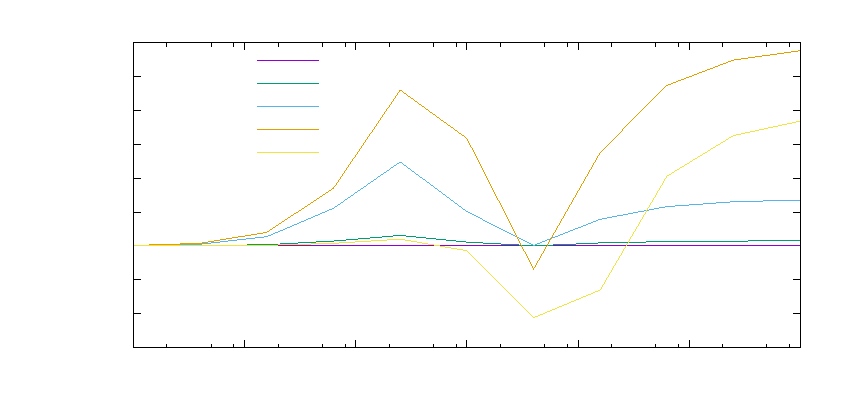
\includegraphics{img/cg1L}}%
    \gplfronttext
  \end{picture}%
\endgroup

\end{subfigure}\\%
\begin{subfigure}[t]{\textwidth}
	% GNUPLOT: LaTeX picture with Postscript
\begingroup
  \makeatletter
  \providecommand\color[2][]{%
    \GenericError{(gnuplot) \space\space\space\@spaces}{%
      Package color not loaded in conjunction with
      terminal option `colourtext'%
    }{See the gnuplot documentation for explanation.%
    }{Either use 'blacktext' in gnuplot or load the package
      color.sty in LaTeX.}%
    \renewcommand\color[2][]{}%
  }%
  \providecommand\includegraphics[2][]{%
    \GenericError{(gnuplot) \space\space\space\@spaces}{%
      Package graphicx or graphics not loaded%
    }{See the gnuplot documentation for explanation.%
    }{The gnuplot epslatex terminal needs graphicx.sty or graphics.sty.}%
    \renewcommand\includegraphics[2][]{}%
  }%
  \providecommand\rotatebox[2]{#2}%
  \@ifundefined{ifGPcolor}{%
    \newif\ifGPcolor
    \GPcolorfalse
  }{}%
  \@ifundefined{ifGPblacktext}{%
    \newif\ifGPblacktext
    \GPblacktexttrue
  }{}%
  % define a \g@addto@macro without @ in the name:
  \let\gplgaddtomacro\g@addto@macro
  % define empty templates for all commands taking text:
  \gdef\gplbacktext{}%
  \gdef\gplfronttext{}%
  \makeatother
  \ifGPblacktext
    % no textcolor at all
    \def\colorrgb#1{}%
    \def\colorgray#1{}%
  \else
    % gray or color?
    \ifGPcolor
      \def\colorrgb#1{\color[rgb]{#1}}%
      \def\colorgray#1{\color[gray]{#1}}%
      \expandafter\def\csname LTw\endcsname{\color{white}}%
      \expandafter\def\csname LTb\endcsname{\color{black}}%
      \expandafter\def\csname LTa\endcsname{\color{black}}%
      \expandafter\def\csname LT0\endcsname{\color[rgb]{1,0,0}}%
      \expandafter\def\csname LT1\endcsname{\color[rgb]{0,1,0}}%
      \expandafter\def\csname LT2\endcsname{\color[rgb]{0,0,1}}%
      \expandafter\def\csname LT3\endcsname{\color[rgb]{1,0,1}}%
      \expandafter\def\csname LT4\endcsname{\color[rgb]{0,1,1}}%
      \expandafter\def\csname LT5\endcsname{\color[rgb]{1,1,0}}%
      \expandafter\def\csname LT6\endcsname{\color[rgb]{0,0,0}}%
      \expandafter\def\csname LT7\endcsname{\color[rgb]{1,0.3,0}}%
      \expandafter\def\csname LT8\endcsname{\color[rgb]{0.5,0.5,0.5}}%
    \else
      % gray
      \def\colorrgb#1{\color{black}}%
      \def\colorgray#1{\color[gray]{#1}}%
      \expandafter\def\csname LTw\endcsname{\color{white}}%
      \expandafter\def\csname LTb\endcsname{\color{black}}%
      \expandafter\def\csname LTa\endcsname{\color{black}}%
      \expandafter\def\csname LT0\endcsname{\color{black}}%
      \expandafter\def\csname LT1\endcsname{\color{black}}%
      \expandafter\def\csname LT2\endcsname{\color{black}}%
      \expandafter\def\csname LT3\endcsname{\color{black}}%
      \expandafter\def\csname LT4\endcsname{\color{black}}%
      \expandafter\def\csname LT5\endcsname{\color{black}}%
      \expandafter\def\csname LT6\endcsname{\color{black}}%
      \expandafter\def\csname LT7\endcsname{\color{black}}%
      \expandafter\def\csname LT8\endcsname{\color{black}}%
    \fi
  \fi
    \setlength{\unitlength}{0.0500bp}%
    \ifx\gptboxheight\undefined%
      \newlength{\gptboxheight}%
      \newlength{\gptboxwidth}%
      \newsavebox{\gptboxtext}%
    \fi%
    \setlength{\fboxrule}{0.5pt}%
    \setlength{\fboxsep}{1pt}%
\begin{picture}(7920.00,3628.80)%
    \gplgaddtomacro\gplbacktext{%
      \csname LTb\endcsname%
      \put(726,440){\makebox(0,0)[r]{\strut{}-0.2}}%
      \put(726,765){\makebox(0,0)[r]{\strut{}-0.1}}%
      \put(726,1090){\makebox(0,0)[r]{\strut{}-0.1}}%
      \put(726,1415){\makebox(0,0)[r]{\strut{}0.0}}%
      \put(726,1740){\makebox(0,0)[r]{\strut{}0.0}}%
      \put(726,2064){\makebox(0,0)[r]{\strut{}0.1}}%
      \put(726,2389){\makebox(0,0)[r]{\strut{}0.1}}%
      \put(726,2714){\makebox(0,0)[r]{\strut{}0.2}}%
      \put(726,3039){\makebox(0,0)[r]{\strut{}0.2}}%
      \put(726,3364){\makebox(0,0)[r]{\strut{}0.3}}%
      \put(858,220){\makebox(0,0){\strut{}$0.001$}}%
      \put(1969,220){\makebox(0,0){\strut{}$0.01$}}%
      \put(3079,220){\makebox(0,0){\strut{}$0.1$}}%
      \put(4190,220){\makebox(0,0){\strut{}$1$}}%
      \put(5301,220){\makebox(0,0){\strut{}$10$}}%
      \put(6411,220){\makebox(0,0){\strut{}$100$}}%
      \put(7522,220){\makebox(0,0){\strut{}$1000$}}%
    }%
    \gplgaddtomacro\gplfronttext{%
      \csname LTb\endcsname%
      \put(5611,3191){\makebox(0,0)[l]{\strut{}$Q^2=10^{-2}$}}%
      \csname LTb\endcsname%
      \put(5611,2971){\makebox(0,0)[l]{\strut{}$Q^2=10^0$}}%
      \csname LTb\endcsname%
      \put(5611,2751){\makebox(0,0)[l]{\strut{}$Q^2=10^1$}}%
      \csname LTb\endcsname%
      \put(5611,2531){\makebox(0,0)[l]{\strut{}$Q^2=10^2$}}%
      \csname LTb\endcsname%
      \put(5611,2311){\makebox(0,0)[l]{\strut{}$Q^2=10^3$}}%
    }%
    \gplbacktext
    \put(0,0){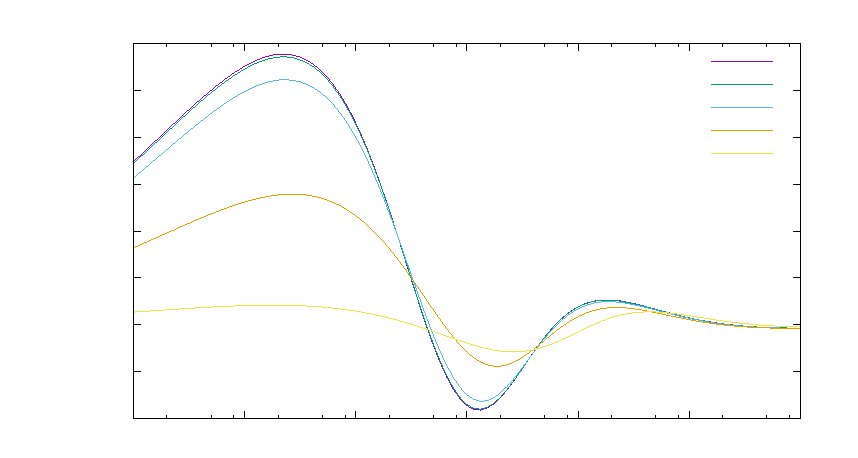
\includegraphics{img/cg1P}}%
    \gplfronttext
  \end{picture}%
\endgroup

\end{subfigure}
\caption{next-to-leading order scaling functions $c_{k,g}^{(1)}(\eta,\xi)$ plotted as function of $\eta=s/(4m^2)-1$ for different values of $Q^2$ in units of $\si{\GeV^2}$ at $m=\SI{4.75}{\GeV}$ (i.e. different values of $\xi=Q^2/m^2$) }\label{fig:cg1}
\end{figure}

\pagebreak
\begin{figure}[ht!]
\centering
\begin{subfigure}[t]{\textwidth}
	% GNUPLOT: LaTeX picture with Postscript
\begingroup
  \makeatletter
  \providecommand\color[2][]{%
    \GenericError{(gnuplot) \space\space\space\@spaces}{%
      Package color not loaded in conjunction with
      terminal option `colourtext'%
    }{See the gnuplot documentation for explanation.%
    }{Either use 'blacktext' in gnuplot or load the package
      color.sty in LaTeX.}%
    \renewcommand\color[2][]{}%
  }%
  \providecommand\includegraphics[2][]{%
    \GenericError{(gnuplot) \space\space\space\@spaces}{%
      Package graphicx or graphics not loaded%
    }{See the gnuplot documentation for explanation.%
    }{The gnuplot epslatex terminal needs graphicx.sty or graphics.sty.}%
    \renewcommand\includegraphics[2][]{}%
  }%
  \providecommand\rotatebox[2]{#2}%
  \@ifundefined{ifGPcolor}{%
    \newif\ifGPcolor
    \GPcolorfalse
  }{}%
  \@ifundefined{ifGPblacktext}{%
    \newif\ifGPblacktext
    \GPblacktexttrue
  }{}%
  % define a \g@addto@macro without @ in the name:
  \let\gplgaddtomacro\g@addto@macro
  % define empty templates for all commands taking text:
  \gdef\gplbacktext{}%
  \gdef\gplfronttext{}%
  \makeatother
  \ifGPblacktext
    % no textcolor at all
    \def\colorrgb#1{}%
    \def\colorgray#1{}%
  \else
    % gray or color?
    \ifGPcolor
      \def\colorrgb#1{\color[rgb]{#1}}%
      \def\colorgray#1{\color[gray]{#1}}%
      \expandafter\def\csname LTw\endcsname{\color{white}}%
      \expandafter\def\csname LTb\endcsname{\color{black}}%
      \expandafter\def\csname LTa\endcsname{\color{black}}%
      \expandafter\def\csname LT0\endcsname{\color[rgb]{1,0,0}}%
      \expandafter\def\csname LT1\endcsname{\color[rgb]{0,1,0}}%
      \expandafter\def\csname LT2\endcsname{\color[rgb]{0,0,1}}%
      \expandafter\def\csname LT3\endcsname{\color[rgb]{1,0,1}}%
      \expandafter\def\csname LT4\endcsname{\color[rgb]{0,1,1}}%
      \expandafter\def\csname LT5\endcsname{\color[rgb]{1,1,0}}%
      \expandafter\def\csname LT6\endcsname{\color[rgb]{0,0,0}}%
      \expandafter\def\csname LT7\endcsname{\color[rgb]{1,0.3,0}}%
      \expandafter\def\csname LT8\endcsname{\color[rgb]{0.5,0.5,0.5}}%
    \else
      % gray
      \def\colorrgb#1{\color{black}}%
      \def\colorgray#1{\color[gray]{#1}}%
      \expandafter\def\csname LTw\endcsname{\color{white}}%
      \expandafter\def\csname LTb\endcsname{\color{black}}%
      \expandafter\def\csname LTa\endcsname{\color{black}}%
      \expandafter\def\csname LT0\endcsname{\color{black}}%
      \expandafter\def\csname LT1\endcsname{\color{black}}%
      \expandafter\def\csname LT2\endcsname{\color{black}}%
      \expandafter\def\csname LT3\endcsname{\color{black}}%
      \expandafter\def\csname LT4\endcsname{\color{black}}%
      \expandafter\def\csname LT5\endcsname{\color{black}}%
      \expandafter\def\csname LT6\endcsname{\color{black}}%
      \expandafter\def\csname LT7\endcsname{\color{black}}%
      \expandafter\def\csname LT8\endcsname{\color{black}}%
    \fi
  \fi
    \setlength{\unitlength}{0.0500bp}%
    \ifx\gptboxheight\undefined%
      \newlength{\gptboxheight}%
      \newlength{\gptboxwidth}%
      \newsavebox{\gptboxtext}%
    \fi%
    \setlength{\fboxrule}{0.5pt}%
    \setlength{\fboxsep}{1pt}%
\begin{picture}(7920.00,3628.80)%
    \gplgaddtomacro\gplbacktext{%
      \csname LTb\endcsname%
      \put(858,440){\makebox(0,0)[r]{\strut{}-0.20}}%
      \put(858,927){\makebox(0,0)[r]{\strut{}-0.15}}%
      \put(858,1415){\makebox(0,0)[r]{\strut{}-0.10}}%
      \put(858,1902){\makebox(0,0)[r]{\strut{}-0.05}}%
      \put(858,2389){\makebox(0,0)[r]{\strut{}0.00}}%
      \put(858,2877){\makebox(0,0)[r]{\strut{}0.05}}%
      \put(858,3364){\makebox(0,0)[r]{\strut{}0.10}}%
      \put(990,220){\makebox(0,0){\strut{}$0.001$}}%
      \put(2079,220){\makebox(0,0){\strut{}$0.01$}}%
      \put(3167,220){\makebox(0,0){\strut{}$0.1$}}%
      \put(4256,220){\makebox(0,0){\strut{}$1$}}%
      \put(5345,220){\makebox(0,0){\strut{}$10$}}%
      \put(6433,220){\makebox(0,0){\strut{}$100$}}%
      \put(7522,220){\makebox(0,0){\strut{}$1000$}}%
    }%
    \gplgaddtomacro\gplfronttext{%
      \csname LTb\endcsname%
      \put(1122,1493){\makebox(0,0)[l]{\strut{}$Q^2=10^{-2}$}}%
      \csname LTb\endcsname%
      \put(1122,1273){\makebox(0,0)[l]{\strut{}$Q^2=10^0$}}%
      \csname LTb\endcsname%
      \put(1122,1053){\makebox(0,0)[l]{\strut{}$Q^2=10^1$}}%
      \csname LTb\endcsname%
      \put(1122,833){\makebox(0,0)[l]{\strut{}$Q^2=10^2$}}%
      \csname LTb\endcsname%
      \put(1122,613){\makebox(0,0)[l]{\strut{}$Q^2=10^3$}}%
    }%
    \gplbacktext
    \put(0,0){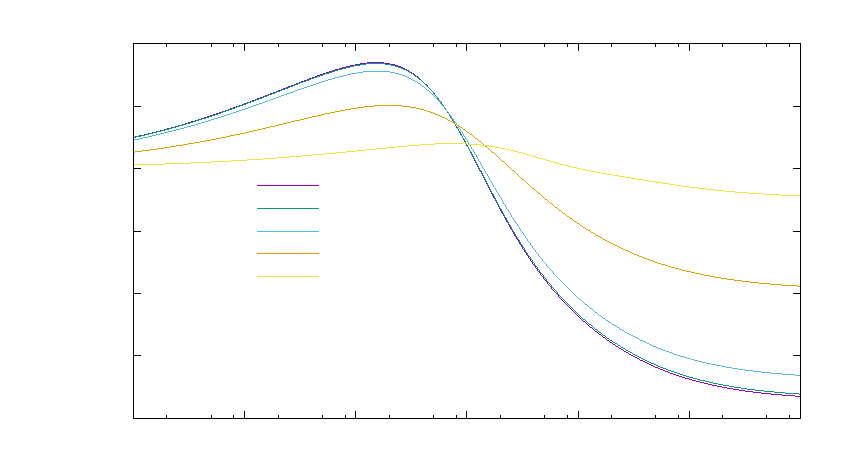
\includegraphics{img/cgBarF1T}}%
    \gplfronttext
  \end{picture}%
\endgroup

\end{subfigure}\\%
\begin{subfigure}[t]{\textwidth}
	% GNUPLOT: LaTeX picture with Postscript
\begingroup
  \makeatletter
  \providecommand\color[2][]{%
    \GenericError{(gnuplot) \space\space\space\@spaces}{%
      Package color not loaded in conjunction with
      terminal option `colourtext'%
    }{See the gnuplot documentation for explanation.%
    }{Either use 'blacktext' in gnuplot or load the package
      color.sty in LaTeX.}%
    \renewcommand\color[2][]{}%
  }%
  \providecommand\includegraphics[2][]{%
    \GenericError{(gnuplot) \space\space\space\@spaces}{%
      Package graphicx or graphics not loaded%
    }{See the gnuplot documentation for explanation.%
    }{The gnuplot epslatex terminal needs graphicx.sty or graphics.sty.}%
    \renewcommand\includegraphics[2][]{}%
  }%
  \providecommand\rotatebox[2]{#2}%
  \@ifundefined{ifGPcolor}{%
    \newif\ifGPcolor
    \GPcolorfalse
  }{}%
  \@ifundefined{ifGPblacktext}{%
    \newif\ifGPblacktext
    \GPblacktexttrue
  }{}%
  % define a \g@addto@macro without @ in the name:
  \let\gplgaddtomacro\g@addto@macro
  % define empty templates for all commands taking text:
  \gdef\gplbacktext{}%
  \gdef\gplfronttext{}%
  \makeatother
  \ifGPblacktext
    % no textcolor at all
    \def\colorrgb#1{}%
    \def\colorgray#1{}%
  \else
    % gray or color?
    \ifGPcolor
      \def\colorrgb#1{\color[rgb]{#1}}%
      \def\colorgray#1{\color[gray]{#1}}%
      \expandafter\def\csname LTw\endcsname{\color{white}}%
      \expandafter\def\csname LTb\endcsname{\color{black}}%
      \expandafter\def\csname LTa\endcsname{\color{black}}%
      \expandafter\def\csname LT0\endcsname{\color[rgb]{1,0,0}}%
      \expandafter\def\csname LT1\endcsname{\color[rgb]{0,1,0}}%
      \expandafter\def\csname LT2\endcsname{\color[rgb]{0,0,1}}%
      \expandafter\def\csname LT3\endcsname{\color[rgb]{1,0,1}}%
      \expandafter\def\csname LT4\endcsname{\color[rgb]{0,1,1}}%
      \expandafter\def\csname LT5\endcsname{\color[rgb]{1,1,0}}%
      \expandafter\def\csname LT6\endcsname{\color[rgb]{0,0,0}}%
      \expandafter\def\csname LT7\endcsname{\color[rgb]{1,0.3,0}}%
      \expandafter\def\csname LT8\endcsname{\color[rgb]{0.5,0.5,0.5}}%
    \else
      % gray
      \def\colorrgb#1{\color{black}}%
      \def\colorgray#1{\color[gray]{#1}}%
      \expandafter\def\csname LTw\endcsname{\color{white}}%
      \expandafter\def\csname LTb\endcsname{\color{black}}%
      \expandafter\def\csname LTa\endcsname{\color{black}}%
      \expandafter\def\csname LT0\endcsname{\color{black}}%
      \expandafter\def\csname LT1\endcsname{\color{black}}%
      \expandafter\def\csname LT2\endcsname{\color{black}}%
      \expandafter\def\csname LT3\endcsname{\color{black}}%
      \expandafter\def\csname LT4\endcsname{\color{black}}%
      \expandafter\def\csname LT5\endcsname{\color{black}}%
      \expandafter\def\csname LT6\endcsname{\color{black}}%
      \expandafter\def\csname LT7\endcsname{\color{black}}%
      \expandafter\def\csname LT8\endcsname{\color{black}}%
    \fi
  \fi
    \setlength{\unitlength}{0.0500bp}%
    \ifx\gptboxheight\undefined%
      \newlength{\gptboxheight}%
      \newlength{\gptboxwidth}%
      \newsavebox{\gptboxtext}%
    \fi%
    \setlength{\fboxrule}{0.5pt}%
    \setlength{\fboxsep}{1pt}%
\begin{picture}(7920.00,4082.40)%
    \gplgaddtomacro\gplbacktext{%
      \csname LTb\endcsname%
      \put(990,220){\makebox(0,0)[r]{\strut{}-0.015}}%
      \put(990,940){\makebox(0,0)[r]{\strut{}-0.010}}%
      \put(990,1659){\makebox(0,0)[r]{\strut{}-0.005}}%
      \put(990,2379){\makebox(0,0)[r]{\strut{}0.000}}%
      \put(990,3098){\makebox(0,0)[r]{\strut{}0.005}}%
      \put(990,3818){\makebox(0,0)[r]{\strut{}0.010}}%
      \put(1122,0){\makebox(0,0){\strut{}$0.001$}}%
      \put(2189,0){\makebox(0,0){\strut{}$0.01$}}%
      \put(3255,0){\makebox(0,0){\strut{}$0.1$}}%
      \put(4322,0){\makebox(0,0){\strut{}$1$}}%
      \put(5389,0){\makebox(0,0){\strut{}$10$}}%
      \put(6455,0){\makebox(0,0){\strut{}$100$}}%
      \put(7522,0){\makebox(0,0){\strut{}$1000$}}%
      \put(1250,472){\makebox(0,0)[l]{\strut{}(b) $\bar c_{L,g}^{F,(1)}(\eta)$}}%
    }%
    \gplgaddtomacro\gplfronttext{%
      \csname LTb\endcsname%
      \put(5611,3645){\makebox(0,0)[l]{\strut{}$Q^2=10^{-2}$}}%
      \csname LTb\endcsname%
      \put(5611,3425){\makebox(0,0)[l]{\strut{}$Q^2=10^0$}}%
      \csname LTb\endcsname%
      \put(5611,3205){\makebox(0,0)[l]{\strut{}$Q^2=10^1$}}%
      \csname LTb\endcsname%
      \put(5611,2985){\makebox(0,0)[l]{\strut{}$Q^2=10^2$}}%
      \csname LTb\endcsname%
      \put(5611,2765){\makebox(0,0)[l]{\strut{}$Q^2=10^3$}}%
    }%
    \gplbacktext
    \put(0,0){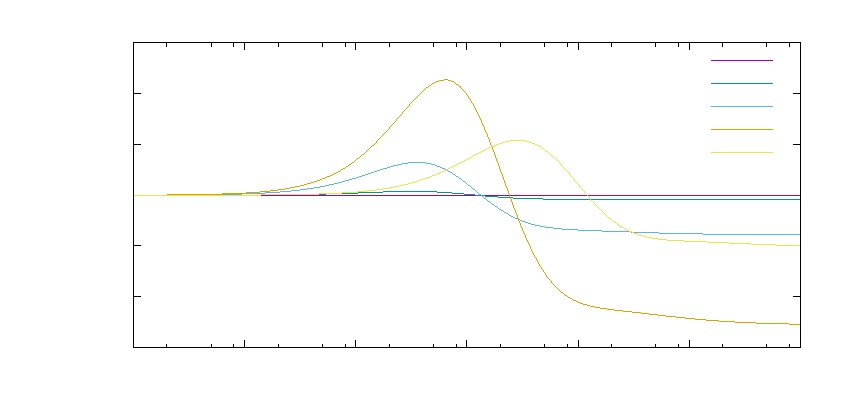
\includegraphics{img/cgBarF1L}}%
    \gplfronttext
  \end{picture}%
\endgroup

\end{subfigure}\\%
\begin{subfigure}[t]{\textwidth}
	% GNUPLOT: LaTeX picture with Postscript
\begingroup
  \makeatletter
  \providecommand\color[2][]{%
    \GenericError{(gnuplot) \space\space\space\@spaces}{%
      Package color not loaded in conjunction with
      terminal option `colourtext'%
    }{See the gnuplot documentation for explanation.%
    }{Either use 'blacktext' in gnuplot or load the package
      color.sty in LaTeX.}%
    \renewcommand\color[2][]{}%
  }%
  \providecommand\includegraphics[2][]{%
    \GenericError{(gnuplot) \space\space\space\@spaces}{%
      Package graphicx or graphics not loaded%
    }{See the gnuplot documentation for explanation.%
    }{The gnuplot epslatex terminal needs graphicx.sty or graphics.sty.}%
    \renewcommand\includegraphics[2][]{}%
  }%
  \providecommand\rotatebox[2]{#2}%
  \@ifundefined{ifGPcolor}{%
    \newif\ifGPcolor
    \GPcolorfalse
  }{}%
  \@ifundefined{ifGPblacktext}{%
    \newif\ifGPblacktext
    \GPblacktexttrue
  }{}%
  % define a \g@addto@macro without @ in the name:
  \let\gplgaddtomacro\g@addto@macro
  % define empty templates for all commands taking text:
  \gdef\gplbacktext{}%
  \gdef\gplfronttext{}%
  \makeatother
  \ifGPblacktext
    % no textcolor at all
    \def\colorrgb#1{}%
    \def\colorgray#1{}%
  \else
    % gray or color?
    \ifGPcolor
      \def\colorrgb#1{\color[rgb]{#1}}%
      \def\colorgray#1{\color[gray]{#1}}%
      \expandafter\def\csname LTw\endcsname{\color{white}}%
      \expandafter\def\csname LTb\endcsname{\color{black}}%
      \expandafter\def\csname LTa\endcsname{\color{black}}%
      \expandafter\def\csname LT0\endcsname{\color[rgb]{1,0,0}}%
      \expandafter\def\csname LT1\endcsname{\color[rgb]{0,1,0}}%
      \expandafter\def\csname LT2\endcsname{\color[rgb]{0,0,1}}%
      \expandafter\def\csname LT3\endcsname{\color[rgb]{1,0,1}}%
      \expandafter\def\csname LT4\endcsname{\color[rgb]{0,1,1}}%
      \expandafter\def\csname LT5\endcsname{\color[rgb]{1,1,0}}%
      \expandafter\def\csname LT6\endcsname{\color[rgb]{0,0,0}}%
      \expandafter\def\csname LT7\endcsname{\color[rgb]{1,0.3,0}}%
      \expandafter\def\csname LT8\endcsname{\color[rgb]{0.5,0.5,0.5}}%
    \else
      % gray
      \def\colorrgb#1{\color{black}}%
      \def\colorgray#1{\color[gray]{#1}}%
      \expandafter\def\csname LTw\endcsname{\color{white}}%
      \expandafter\def\csname LTb\endcsname{\color{black}}%
      \expandafter\def\csname LTa\endcsname{\color{black}}%
      \expandafter\def\csname LT0\endcsname{\color{black}}%
      \expandafter\def\csname LT1\endcsname{\color{black}}%
      \expandafter\def\csname LT2\endcsname{\color{black}}%
      \expandafter\def\csname LT3\endcsname{\color{black}}%
      \expandafter\def\csname LT4\endcsname{\color{black}}%
      \expandafter\def\csname LT5\endcsname{\color{black}}%
      \expandafter\def\csname LT6\endcsname{\color{black}}%
      \expandafter\def\csname LT7\endcsname{\color{black}}%
      \expandafter\def\csname LT8\endcsname{\color{black}}%
    \fi
  \fi
    \setlength{\unitlength}{0.0500bp}%
    \ifx\gptboxheight\undefined%
      \newlength{\gptboxheight}%
      \newlength{\gptboxwidth}%
      \newsavebox{\gptboxtext}%
    \fi%
    \setlength{\fboxrule}{0.5pt}%
    \setlength{\fboxsep}{1pt}%
\begin{picture}(7920.00,4082.40)%
    \gplgaddtomacro\gplbacktext{%
      \csname LTb\endcsname%
      \put(990,220){\makebox(0,0)[r]{\strut{} -0.04}}%
      \put(990,580){\makebox(0,0)[r]{\strut{} -0.03}}%
      \put(990,940){\makebox(0,0)[r]{\strut{} -0.02}}%
      \put(990,1299){\makebox(0,0)[r]{\strut{} -0.01}}%
      \put(990,1659){\makebox(0,0)[r]{\strut{} 0.00}}%
      \put(990,2019){\makebox(0,0)[r]{\strut{} 0.01}}%
      \put(990,2379){\makebox(0,0)[r]{\strut{} 0.02}}%
      \put(990,2739){\makebox(0,0)[r]{\strut{} 0.03}}%
      \put(990,3098){\makebox(0,0)[r]{\strut{} 0.04}}%
      \put(990,3458){\makebox(0,0)[r]{\strut{} 0.05}}%
      \put(990,3818){\makebox(0,0)[r]{\strut{} 0.06}}%
      \put(1122,0){\makebox(0,0){\strut{}$0.001$}}%
      \put(2189,0){\makebox(0,0){\strut{}$0.01$}}%
      \put(3255,0){\makebox(0,0){\strut{}$0.1$}}%
      \put(4322,0){\makebox(0,0){\strut{}$1$}}%
      \put(5389,0){\makebox(0,0){\strut{}$10$}}%
      \put(6455,0){\makebox(0,0){\strut{}$100$}}%
      \put(7522,0){\makebox(0,0){\strut{}$1000$}}%
      \put(1250,472){\makebox(0,0)[l]{\strut{}(c) $\bar c_{P,g}^{F,(1)}(\eta)$}}%
    }%
    \gplgaddtomacro\gplfronttext{%
      \csname LTb\endcsname%
      \put(5611,3645){\makebox(0,0)[l]{\strut{}$Q^2=10^{-2}$}}%
      \csname LTb\endcsname%
      \put(5611,3425){\makebox(0,0)[l]{\strut{}$Q^2=10^0$}}%
      \csname LTb\endcsname%
      \put(5611,3205){\makebox(0,0)[l]{\strut{}$Q^2=10^1$}}%
      \csname LTb\endcsname%
      \put(5611,2985){\makebox(0,0)[l]{\strut{}$Q^2=10^2$}}%
      \csname LTb\endcsname%
      \put(5611,2765){\makebox(0,0)[l]{\strut{}$Q^2=10^3$}}%
    }%
    \gplbacktext
    \put(0,0){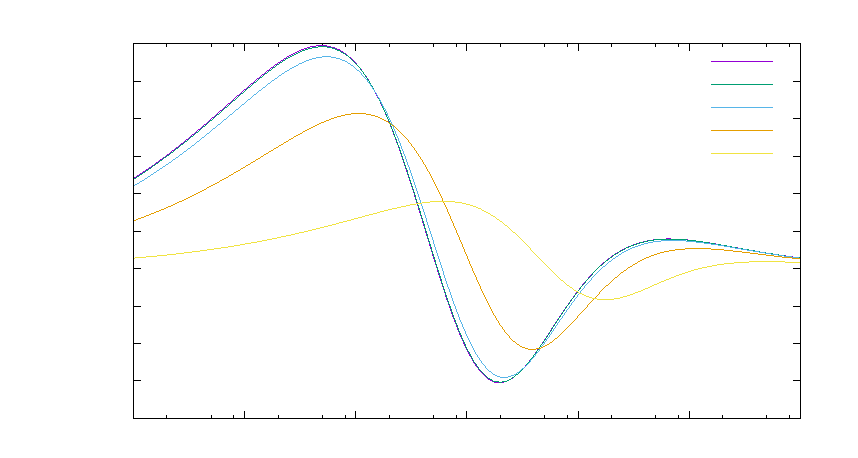
\includegraphics{img/cgBarF1P}}%
    \gplfronttext
  \end{picture}%
\endgroup

\end{subfigure}
\caption{next-to-leading order scaling functions $\bar c_{k,g}^{F,(1)}(\eta,\xi)$ plotted as function of $\eta=s/(4m^2)-1$ for different values of $Q^2$ in units of $\si{\GeV^2}$ at $m=\SI{4.75}{\GeV}$ (i.e. different values of $\xi=Q^2/m^2$) and $n_{lf}=4$ }\label{fig:cgBarF1}
\end{figure}

\pagebreak
\begin{figure}[ht!]
\centering
\begin{subfigure}[t]{\textwidth}
	% GNUPLOT: LaTeX picture with Postscript
\begingroup
  \makeatletter
  \providecommand\color[2][]{%
    \GenericError{(gnuplot) \space\space\space\@spaces}{%
      Package color not loaded in conjunction with
      terminal option `colourtext'%
    }{See the gnuplot documentation for explanation.%
    }{Either use 'blacktext' in gnuplot or load the package
      color.sty in LaTeX.}%
    \renewcommand\color[2][]{}%
  }%
  \providecommand\includegraphics[2][]{%
    \GenericError{(gnuplot) \space\space\space\@spaces}{%
      Package graphicx or graphics not loaded%
    }{See the gnuplot documentation for explanation.%
    }{The gnuplot epslatex terminal needs graphicx.sty or graphics.sty.}%
    \renewcommand\includegraphics[2][]{}%
  }%
  \providecommand\rotatebox[2]{#2}%
  \@ifundefined{ifGPcolor}{%
    \newif\ifGPcolor
    \GPcolorfalse
  }{}%
  \@ifundefined{ifGPblacktext}{%
    \newif\ifGPblacktext
    \GPblacktexttrue
  }{}%
  % define a \g@addto@macro without @ in the name:
  \let\gplgaddtomacro\g@addto@macro
  % define empty templates for all commands taking text:
  \gdef\gplbacktext{}%
  \gdef\gplfronttext{}%
  \makeatother
  \ifGPblacktext
    % no textcolor at all
    \def\colorrgb#1{}%
    \def\colorgray#1{}%
  \else
    % gray or color?
    \ifGPcolor
      \def\colorrgb#1{\color[rgb]{#1}}%
      \def\colorgray#1{\color[gray]{#1}}%
      \expandafter\def\csname LTw\endcsname{\color{white}}%
      \expandafter\def\csname LTb\endcsname{\color{black}}%
      \expandafter\def\csname LTa\endcsname{\color{black}}%
      \expandafter\def\csname LT0\endcsname{\color[rgb]{1,0,0}}%
      \expandafter\def\csname LT1\endcsname{\color[rgb]{0,1,0}}%
      \expandafter\def\csname LT2\endcsname{\color[rgb]{0,0,1}}%
      \expandafter\def\csname LT3\endcsname{\color[rgb]{1,0,1}}%
      \expandafter\def\csname LT4\endcsname{\color[rgb]{0,1,1}}%
      \expandafter\def\csname LT5\endcsname{\color[rgb]{1,1,0}}%
      \expandafter\def\csname LT6\endcsname{\color[rgb]{0,0,0}}%
      \expandafter\def\csname LT7\endcsname{\color[rgb]{1,0.3,0}}%
      \expandafter\def\csname LT8\endcsname{\color[rgb]{0.5,0.5,0.5}}%
    \else
      % gray
      \def\colorrgb#1{\color{black}}%
      \def\colorgray#1{\color[gray]{#1}}%
      \expandafter\def\csname LTw\endcsname{\color{white}}%
      \expandafter\def\csname LTb\endcsname{\color{black}}%
      \expandafter\def\csname LTa\endcsname{\color{black}}%
      \expandafter\def\csname LT0\endcsname{\color{black}}%
      \expandafter\def\csname LT1\endcsname{\color{black}}%
      \expandafter\def\csname LT2\endcsname{\color{black}}%
      \expandafter\def\csname LT3\endcsname{\color{black}}%
      \expandafter\def\csname LT4\endcsname{\color{black}}%
      \expandafter\def\csname LT5\endcsname{\color{black}}%
      \expandafter\def\csname LT6\endcsname{\color{black}}%
      \expandafter\def\csname LT7\endcsname{\color{black}}%
      \expandafter\def\csname LT8\endcsname{\color{black}}%
    \fi
  \fi
    \setlength{\unitlength}{0.0500bp}%
    \ifx\gptboxheight\undefined%
      \newlength{\gptboxheight}%
      \newlength{\gptboxwidth}%
      \newsavebox{\gptboxtext}%
    \fi%
    \setlength{\fboxrule}{0.5pt}%
    \setlength{\fboxsep}{1pt}%
\begin{picture}(7920.00,4082.40)%
    \gplgaddtomacro\gplbacktext{%
      \csname LTb\endcsname%
      \put(726,220){\makebox(0,0)[r]{\strut{}0.00}}%
      \put(726,580){\makebox(0,0)[r]{\strut{}0.01}}%
      \put(726,940){\makebox(0,0)[r]{\strut{}0.02}}%
      \put(726,1299){\makebox(0,0)[r]{\strut{}0.03}}%
      \put(726,1659){\makebox(0,0)[r]{\strut{}0.04}}%
      \put(726,2019){\makebox(0,0)[r]{\strut{}0.05}}%
      \put(726,2379){\makebox(0,0)[r]{\strut{}0.06}}%
      \put(726,2739){\makebox(0,0)[r]{\strut{}0.07}}%
      \put(726,3098){\makebox(0,0)[r]{\strut{}0.08}}%
      \put(726,3458){\makebox(0,0)[r]{\strut{}0.09}}%
      \put(726,3818){\makebox(0,0)[r]{\strut{}0.10}}%
      \put(858,0){\makebox(0,0){\strut{}$0.001$}}%
      \put(1969,0){\makebox(0,0){\strut{}$0.01$}}%
      \put(3079,0){\makebox(0,0){\strut{}$0.1$}}%
      \put(4190,0){\makebox(0,0){\strut{}$1$}}%
      \put(5301,0){\makebox(0,0){\strut{}$10$}}%
      \put(6411,0){\makebox(0,0){\strut{}$100$}}%
      \put(7522,0){\makebox(0,0){\strut{}$1000$}}%
      \put(991,3458){\makebox(0,0)[l]{\strut{}(a) $\bar c_{T,g}^{R,(1)}(\eta)$}}%
    }%
    \gplgaddtomacro\gplfronttext{%
      \csname LTb\endcsname%
      \put(5611,3645){\makebox(0,0)[l]{\strut{}$Q^2=10^{-2}$}}%
      \csname LTb\endcsname%
      \put(5611,3425){\makebox(0,0)[l]{\strut{}$Q^2=10^0$}}%
      \csname LTb\endcsname%
      \put(5611,3205){\makebox(0,0)[l]{\strut{}$Q^2=10^1$}}%
      \csname LTb\endcsname%
      \put(5611,2985){\makebox(0,0)[l]{\strut{}$Q^2=10^2$}}%
      \csname LTb\endcsname%
      \put(5611,2765){\makebox(0,0)[l]{\strut{}$Q^2=10^3$}}%
    }%
    \gplbacktext
    \put(0,0){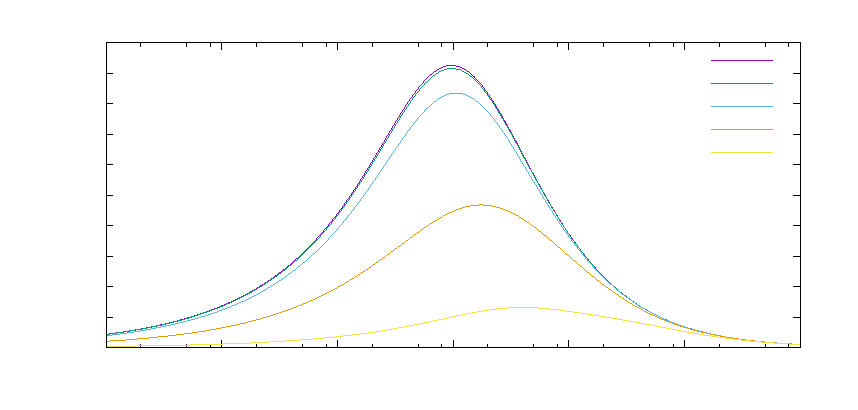
\includegraphics{img/cgBarR1T}}%
    \gplfronttext
  \end{picture}%
\endgroup

\end{subfigure}\\%
\begin{subfigure}[t]{\textwidth}
	% GNUPLOT: LaTeX picture with Postscript
\begingroup
  \makeatletter
  \providecommand\color[2][]{%
    \GenericError{(gnuplot) \space\space\space\@spaces}{%
      Package color not loaded in conjunction with
      terminal option `colourtext'%
    }{See the gnuplot documentation for explanation.%
    }{Either use 'blacktext' in gnuplot or load the package
      color.sty in LaTeX.}%
    \renewcommand\color[2][]{}%
  }%
  \providecommand\includegraphics[2][]{%
    \GenericError{(gnuplot) \space\space\space\@spaces}{%
      Package graphicx or graphics not loaded%
    }{See the gnuplot documentation for explanation.%
    }{The gnuplot epslatex terminal needs graphicx.sty or graphics.sty.}%
    \renewcommand\includegraphics[2][]{}%
  }%
  \providecommand\rotatebox[2]{#2}%
  \@ifundefined{ifGPcolor}{%
    \newif\ifGPcolor
    \GPcolorfalse
  }{}%
  \@ifundefined{ifGPblacktext}{%
    \newif\ifGPblacktext
    \GPblacktexttrue
  }{}%
  % define a \g@addto@macro without @ in the name:
  \let\gplgaddtomacro\g@addto@macro
  % define empty templates for all commands taking text:
  \gdef\gplbacktext{}%
  \gdef\gplfronttext{}%
  \makeatother
  \ifGPblacktext
    % no textcolor at all
    \def\colorrgb#1{}%
    \def\colorgray#1{}%
  \else
    % gray or color?
    \ifGPcolor
      \def\colorrgb#1{\color[rgb]{#1}}%
      \def\colorgray#1{\color[gray]{#1}}%
      \expandafter\def\csname LTw\endcsname{\color{white}}%
      \expandafter\def\csname LTb\endcsname{\color{black}}%
      \expandafter\def\csname LTa\endcsname{\color{black}}%
      \expandafter\def\csname LT0\endcsname{\color[rgb]{1,0,0}}%
      \expandafter\def\csname LT1\endcsname{\color[rgb]{0,1,0}}%
      \expandafter\def\csname LT2\endcsname{\color[rgb]{0,0,1}}%
      \expandafter\def\csname LT3\endcsname{\color[rgb]{1,0,1}}%
      \expandafter\def\csname LT4\endcsname{\color[rgb]{0,1,1}}%
      \expandafter\def\csname LT5\endcsname{\color[rgb]{1,1,0}}%
      \expandafter\def\csname LT6\endcsname{\color[rgb]{0,0,0}}%
      \expandafter\def\csname LT7\endcsname{\color[rgb]{1,0.3,0}}%
      \expandafter\def\csname LT8\endcsname{\color[rgb]{0.5,0.5,0.5}}%
    \else
      % gray
      \def\colorrgb#1{\color{black}}%
      \def\colorgray#1{\color[gray]{#1}}%
      \expandafter\def\csname LTw\endcsname{\color{white}}%
      \expandafter\def\csname LTb\endcsname{\color{black}}%
      \expandafter\def\csname LTa\endcsname{\color{black}}%
      \expandafter\def\csname LT0\endcsname{\color{black}}%
      \expandafter\def\csname LT1\endcsname{\color{black}}%
      \expandafter\def\csname LT2\endcsname{\color{black}}%
      \expandafter\def\csname LT3\endcsname{\color{black}}%
      \expandafter\def\csname LT4\endcsname{\color{black}}%
      \expandafter\def\csname LT5\endcsname{\color{black}}%
      \expandafter\def\csname LT6\endcsname{\color{black}}%
      \expandafter\def\csname LT7\endcsname{\color{black}}%
      \expandafter\def\csname LT8\endcsname{\color{black}}%
    \fi
  \fi
    \setlength{\unitlength}{0.0500bp}%
    \ifx\gptboxheight\undefined%
      \newlength{\gptboxheight}%
      \newlength{\gptboxwidth}%
      \newsavebox{\gptboxtext}%
    \fi%
    \setlength{\fboxrule}{0.5pt}%
    \setlength{\fboxsep}{1pt}%
\begin{picture}(7920.00,3628.80)%
    \gplgaddtomacro\gplbacktext{%
      \csname LTb\endcsname%
      \put(858,440){\makebox(0,0)[r]{\strut{}0.000}}%
      \put(858,927){\makebox(0,0)[r]{\strut{}0.002}}%
      \put(858,1415){\makebox(0,0)[r]{\strut{}0.004}}%
      \put(858,1902){\makebox(0,0)[r]{\strut{}0.006}}%
      \put(858,2389){\makebox(0,0)[r]{\strut{}0.008}}%
      \put(858,2877){\makebox(0,0)[r]{\strut{}0.010}}%
      \put(858,3364){\makebox(0,0)[r]{\strut{}0.012}}%
      \put(990,220){\makebox(0,0){\strut{}$0.001$}}%
      \put(2079,220){\makebox(0,0){\strut{}$0.01$}}%
      \put(3167,220){\makebox(0,0){\strut{}$0.1$}}%
      \put(4256,220){\makebox(0,0){\strut{}$1$}}%
      \put(5345,220){\makebox(0,0){\strut{}$10$}}%
      \put(6433,220){\makebox(0,0){\strut{}$100$}}%
      \put(7522,220){\makebox(0,0){\strut{}$1000$}}%
    }%
    \gplgaddtomacro\gplfronttext{%
      \csname LTb\endcsname%
      \put(5611,3191){\makebox(0,0)[l]{\strut{}$Q^2=10^{-2}$}}%
      \csname LTb\endcsname%
      \put(5611,2971){\makebox(0,0)[l]{\strut{}$Q^2=10^0$}}%
      \csname LTb\endcsname%
      \put(5611,2751){\makebox(0,0)[l]{\strut{}$Q^2=10^1$}}%
      \csname LTb\endcsname%
      \put(5611,2531){\makebox(0,0)[l]{\strut{}$Q^2=10^2$}}%
      \csname LTb\endcsname%
      \put(5611,2311){\makebox(0,0)[l]{\strut{}$Q^2=10^3$}}%
    }%
    \gplbacktext
    \put(0,0){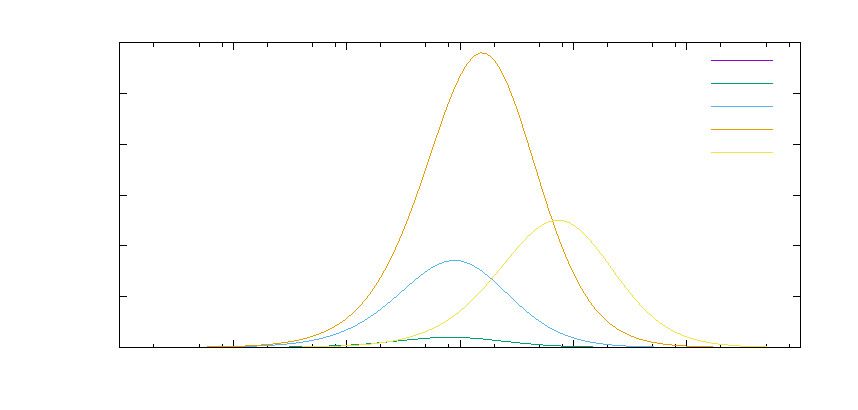
\includegraphics{img/cgBarR1L}}%
    \gplfronttext
  \end{picture}%
\endgroup

\end{subfigure}\\%
\begin{subfigure}[t]{\textwidth}
	% GNUPLOT: LaTeX picture with Postscript
\begingroup
  \makeatletter
  \providecommand\color[2][]{%
    \GenericError{(gnuplot) \space\space\space\@spaces}{%
      Package color not loaded in conjunction with
      terminal option `colourtext'%
    }{See the gnuplot documentation for explanation.%
    }{Either use 'blacktext' in gnuplot or load the package
      color.sty in LaTeX.}%
    \renewcommand\color[2][]{}%
  }%
  \providecommand\includegraphics[2][]{%
    \GenericError{(gnuplot) \space\space\space\@spaces}{%
      Package graphicx or graphics not loaded%
    }{See the gnuplot documentation for explanation.%
    }{The gnuplot epslatex terminal needs graphicx.sty or graphics.sty.}%
    \renewcommand\includegraphics[2][]{}%
  }%
  \providecommand\rotatebox[2]{#2}%
  \@ifundefined{ifGPcolor}{%
    \newif\ifGPcolor
    \GPcolorfalse
  }{}%
  \@ifundefined{ifGPblacktext}{%
    \newif\ifGPblacktext
    \GPblacktexttrue
  }{}%
  % define a \g@addto@macro without @ in the name:
  \let\gplgaddtomacro\g@addto@macro
  % define empty templates for all commands taking text:
  \gdef\gplbacktext{}%
  \gdef\gplfronttext{}%
  \makeatother
  \ifGPblacktext
    % no textcolor at all
    \def\colorrgb#1{}%
    \def\colorgray#1{}%
  \else
    % gray or color?
    \ifGPcolor
      \def\colorrgb#1{\color[rgb]{#1}}%
      \def\colorgray#1{\color[gray]{#1}}%
      \expandafter\def\csname LTw\endcsname{\color{white}}%
      \expandafter\def\csname LTb\endcsname{\color{black}}%
      \expandafter\def\csname LTa\endcsname{\color{black}}%
      \expandafter\def\csname LT0\endcsname{\color[rgb]{1,0,0}}%
      \expandafter\def\csname LT1\endcsname{\color[rgb]{0,1,0}}%
      \expandafter\def\csname LT2\endcsname{\color[rgb]{0,0,1}}%
      \expandafter\def\csname LT3\endcsname{\color[rgb]{1,0,1}}%
      \expandafter\def\csname LT4\endcsname{\color[rgb]{0,1,1}}%
      \expandafter\def\csname LT5\endcsname{\color[rgb]{1,1,0}}%
      \expandafter\def\csname LT6\endcsname{\color[rgb]{0,0,0}}%
      \expandafter\def\csname LT7\endcsname{\color[rgb]{1,0.3,0}}%
      \expandafter\def\csname LT8\endcsname{\color[rgb]{0.5,0.5,0.5}}%
    \else
      % gray
      \def\colorrgb#1{\color{black}}%
      \def\colorgray#1{\color[gray]{#1}}%
      \expandafter\def\csname LTw\endcsname{\color{white}}%
      \expandafter\def\csname LTb\endcsname{\color{black}}%
      \expandafter\def\csname LTa\endcsname{\color{black}}%
      \expandafter\def\csname LT0\endcsname{\color{black}}%
      \expandafter\def\csname LT1\endcsname{\color{black}}%
      \expandafter\def\csname LT2\endcsname{\color{black}}%
      \expandafter\def\csname LT3\endcsname{\color{black}}%
      \expandafter\def\csname LT4\endcsname{\color{black}}%
      \expandafter\def\csname LT5\endcsname{\color{black}}%
      \expandafter\def\csname LT6\endcsname{\color{black}}%
      \expandafter\def\csname LT7\endcsname{\color{black}}%
      \expandafter\def\csname LT8\endcsname{\color{black}}%
    \fi
  \fi
    \setlength{\unitlength}{0.0500bp}%
    \ifx\gptboxheight\undefined%
      \newlength{\gptboxheight}%
      \newlength{\gptboxwidth}%
      \newsavebox{\gptboxtext}%
    \fi%
    \setlength{\fboxrule}{0.5pt}%
    \setlength{\fboxsep}{1pt}%
\begin{picture}(7920.00,4082.40)%
    \gplgaddtomacro\gplbacktext{%
      \csname LTb\endcsname%
      \put(858,220){\makebox(0,0)[r]{\strut{}-0.02}}%
      \put(858,734){\makebox(0,0)[r]{\strut{}-0.01}}%
      \put(858,1248){\makebox(0,0)[r]{\strut{}0.00}}%
      \put(858,1762){\makebox(0,0)[r]{\strut{}0.01}}%
      \put(858,2276){\makebox(0,0)[r]{\strut{}0.02}}%
      \put(858,2790){\makebox(0,0)[r]{\strut{}0.03}}%
      \put(858,3304){\makebox(0,0)[r]{\strut{}0.04}}%
      \put(858,3818){\makebox(0,0)[r]{\strut{}0.05}}%
      \put(990,0){\makebox(0,0){\strut{}$0.001$}}%
      \put(2079,0){\makebox(0,0){\strut{}$0.01$}}%
      \put(3167,0){\makebox(0,0){\strut{}$0.1$}}%
      \put(4256,0){\makebox(0,0){\strut{}$1$}}%
      \put(5345,0){\makebox(0,0){\strut{}$10$}}%
      \put(6433,0){\makebox(0,0){\strut{}$100$}}%
      \put(7522,0){\makebox(0,0){\strut{}$1000$}}%
      \put(1121,3458){\makebox(0,0)[l]{\strut{}(c) $\bar c_{P,g}^{R,(1)}(\eta)$}}%
    }%
    \gplgaddtomacro\gplfronttext{%
      \csname LTb\endcsname%
      \put(5611,3645){\makebox(0,0)[l]{\strut{}$Q^2=10^{-2}$}}%
      \csname LTb\endcsname%
      \put(5611,3425){\makebox(0,0)[l]{\strut{}$Q^2=10^0$}}%
      \csname LTb\endcsname%
      \put(5611,3205){\makebox(0,0)[l]{\strut{}$Q^2=10^1$}}%
      \csname LTb\endcsname%
      \put(5611,2985){\makebox(0,0)[l]{\strut{}$Q^2=10^2$}}%
      \csname LTb\endcsname%
      \put(5611,2765){\makebox(0,0)[l]{\strut{}$Q^2=10^3$}}%
    }%
    \gplbacktext
    \put(0,0){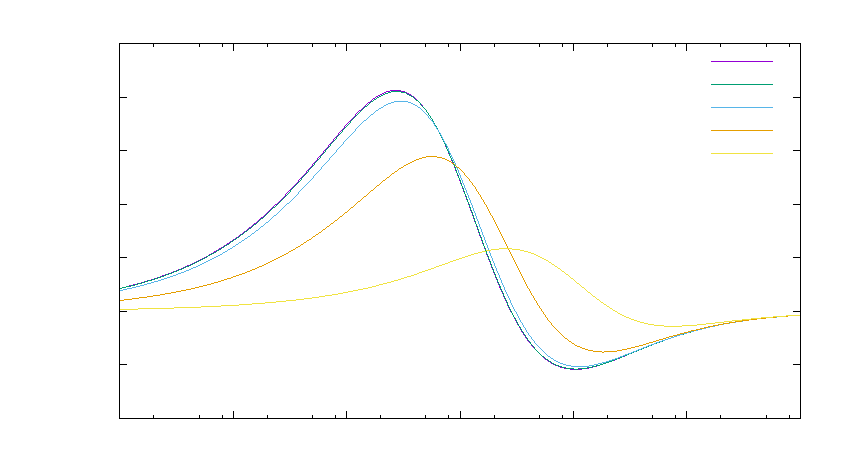
\includegraphics{img/cgBarR1P}}%
    \gplfronttext
  \end{picture}%
\endgroup

\end{subfigure}
\caption{next-to-leading order scaling functions $\bar c_{k,g}^{R,(1)}(\eta,\xi)$ plotted as function of $\eta=s/(4m^2)-1$ for different values of $Q^2$ in units of $\si{\GeV^2}$ at $m=\SI{4.75}{\GeV}$ (i.e. different values of $\xi=Q^2/m^2$)}\label{fig:cgBarR1}
\end{figure}

\pagebreak
\begin{figure}[ht!]
\centering
\begin{subfigure}[t]{\textwidth}
	% GNUPLOT: LaTeX picture with Postscript
\begingroup
  \makeatletter
  \providecommand\color[2][]{%
    \GenericError{(gnuplot) \space\space\space\@spaces}{%
      Package color not loaded in conjunction with
      terminal option `colourtext'%
    }{See the gnuplot documentation for explanation.%
    }{Either use 'blacktext' in gnuplot or load the package
      color.sty in LaTeX.}%
    \renewcommand\color[2][]{}%
  }%
  \providecommand\includegraphics[2][]{%
    \GenericError{(gnuplot) \space\space\space\@spaces}{%
      Package graphicx or graphics not loaded%
    }{See the gnuplot documentation for explanation.%
    }{The gnuplot epslatex terminal needs graphicx.sty or graphics.sty.}%
    \renewcommand\includegraphics[2][]{}%
  }%
  \providecommand\rotatebox[2]{#2}%
  \@ifundefined{ifGPcolor}{%
    \newif\ifGPcolor
    \GPcolorfalse
  }{}%
  \@ifundefined{ifGPblacktext}{%
    \newif\ifGPblacktext
    \GPblacktexttrue
  }{}%
  % define a \g@addto@macro without @ in the name:
  \let\gplgaddtomacro\g@addto@macro
  % define empty templates for all commands taking text:
  \gdef\gplbacktext{}%
  \gdef\gplfronttext{}%
  \makeatother
  \ifGPblacktext
    % no textcolor at all
    \def\colorrgb#1{}%
    \def\colorgray#1{}%
  \else
    % gray or color?
    \ifGPcolor
      \def\colorrgb#1{\color[rgb]{#1}}%
      \def\colorgray#1{\color[gray]{#1}}%
      \expandafter\def\csname LTw\endcsname{\color{white}}%
      \expandafter\def\csname LTb\endcsname{\color{black}}%
      \expandafter\def\csname LTa\endcsname{\color{black}}%
      \expandafter\def\csname LT0\endcsname{\color[rgb]{1,0,0}}%
      \expandafter\def\csname LT1\endcsname{\color[rgb]{0,1,0}}%
      \expandafter\def\csname LT2\endcsname{\color[rgb]{0,0,1}}%
      \expandafter\def\csname LT3\endcsname{\color[rgb]{1,0,1}}%
      \expandafter\def\csname LT4\endcsname{\color[rgb]{0,1,1}}%
      \expandafter\def\csname LT5\endcsname{\color[rgb]{1,1,0}}%
      \expandafter\def\csname LT6\endcsname{\color[rgb]{0,0,0}}%
      \expandafter\def\csname LT7\endcsname{\color[rgb]{1,0.3,0}}%
      \expandafter\def\csname LT8\endcsname{\color[rgb]{0.5,0.5,0.5}}%
    \else
      % gray
      \def\colorrgb#1{\color{black}}%
      \def\colorgray#1{\color[gray]{#1}}%
      \expandafter\def\csname LTw\endcsname{\color{white}}%
      \expandafter\def\csname LTb\endcsname{\color{black}}%
      \expandafter\def\csname LTa\endcsname{\color{black}}%
      \expandafter\def\csname LT0\endcsname{\color{black}}%
      \expandafter\def\csname LT1\endcsname{\color{black}}%
      \expandafter\def\csname LT2\endcsname{\color{black}}%
      \expandafter\def\csname LT3\endcsname{\color{black}}%
      \expandafter\def\csname LT4\endcsname{\color{black}}%
      \expandafter\def\csname LT5\endcsname{\color{black}}%
      \expandafter\def\csname LT6\endcsname{\color{black}}%
      \expandafter\def\csname LT7\endcsname{\color{black}}%
      \expandafter\def\csname LT8\endcsname{\color{black}}%
    \fi
  \fi
    \setlength{\unitlength}{0.0500bp}%
    \ifx\gptboxheight\undefined%
      \newlength{\gptboxheight}%
      \newlength{\gptboxwidth}%
      \newsavebox{\gptboxtext}%
    \fi%
    \setlength{\fboxrule}{0.5pt}%
    \setlength{\fboxsep}{1pt}%
\begin{picture}(7920.00,4082.40)%
    \gplgaddtomacro\gplbacktext{%
      \csname LTb\endcsname%
      \put(990,220){\makebox(0,0)[r]{\strut{} -0.20}}%
      \put(990,734){\makebox(0,0)[r]{\strut{} -0.15}}%
      \put(990,1248){\makebox(0,0)[r]{\strut{} -0.10}}%
      \put(990,1762){\makebox(0,0)[r]{\strut{} -0.05}}%
      \put(990,2276){\makebox(0,0)[r]{\strut{} 0.00}}%
      \put(990,2790){\makebox(0,0)[r]{\strut{} 0.05}}%
      \put(990,3304){\makebox(0,0)[r]{\strut{} 0.10}}%
      \put(990,3818){\makebox(0,0)[r]{\strut{} 0.15}}%
      \put(1122,0){\makebox(0,0){\strut{}$0.001$}}%
      \put(2189,0){\makebox(0,0){\strut{}$0.01$}}%
      \put(3255,0){\makebox(0,0){\strut{}$0.1$}}%
      \put(4322,0){\makebox(0,0){\strut{}$1$}}%
      \put(5389,0){\makebox(0,0){\strut{}$10$}}%
      \put(6455,0){\makebox(0,0){\strut{}$100$}}%
      \put(7522,0){\makebox(0,0){\strut{}$1000$}}%
      \put(1250,3458){\makebox(0,0)[l]{\strut{}(a) $\bar c_{T,g}^{(1)}(\eta)$}}%
    }%
    \gplgaddtomacro\gplfronttext{%
      \csname LTb\endcsname%
      \put(5611,3645){\makebox(0,0)[l]{\strut{}$Q^2=10^{-2}$}}%
      \csname LTb\endcsname%
      \put(5611,3425){\makebox(0,0)[l]{\strut{}$Q^2=10^0$}}%
      \csname LTb\endcsname%
      \put(5611,3205){\makebox(0,0)[l]{\strut{}$Q^2=10^1$}}%
      \csname LTb\endcsname%
      \put(5611,2985){\makebox(0,0)[l]{\strut{}$Q^2=10^2$}}%
      \csname LTb\endcsname%
      \put(5611,2765){\makebox(0,0)[l]{\strut{}$Q^2=10^3$}}%
    }%
    \gplbacktext
    \put(0,0){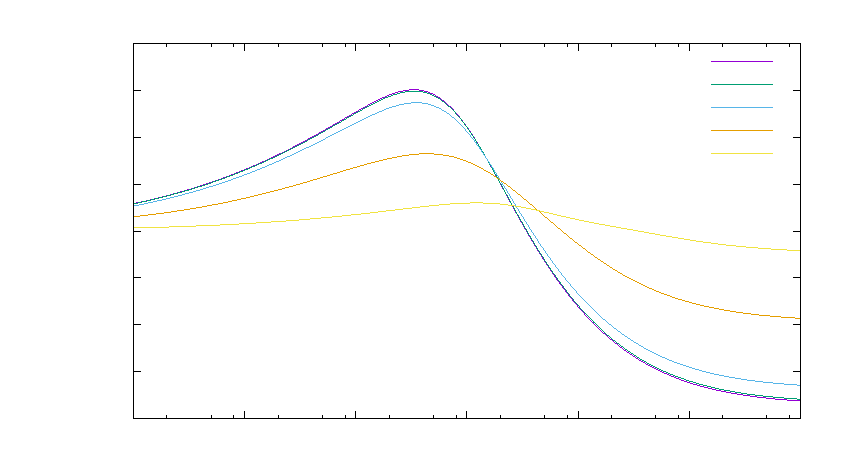
\includegraphics{img/cgBar1T}}%
    \gplfronttext
  \end{picture}%
\endgroup

\end{subfigure}\\%
\begin{subfigure}[t]{\textwidth}
	% GNUPLOT: LaTeX picture with Postscript
\begingroup
  \makeatletter
  \providecommand\color[2][]{%
    \GenericError{(gnuplot) \space\space\space\@spaces}{%
      Package color not loaded in conjunction with
      terminal option `colourtext'%
    }{See the gnuplot documentation for explanation.%
    }{Either use 'blacktext' in gnuplot or load the package
      color.sty in LaTeX.}%
    \renewcommand\color[2][]{}%
  }%
  \providecommand\includegraphics[2][]{%
    \GenericError{(gnuplot) \space\space\space\@spaces}{%
      Package graphicx or graphics not loaded%
    }{See the gnuplot documentation for explanation.%
    }{The gnuplot epslatex terminal needs graphicx.sty or graphics.sty.}%
    \renewcommand\includegraphics[2][]{}%
  }%
  \providecommand\rotatebox[2]{#2}%
  \@ifundefined{ifGPcolor}{%
    \newif\ifGPcolor
    \GPcolorfalse
  }{}%
  \@ifundefined{ifGPblacktext}{%
    \newif\ifGPblacktext
    \GPblacktexttrue
  }{}%
  % define a \g@addto@macro without @ in the name:
  \let\gplgaddtomacro\g@addto@macro
  % define empty templates for all commands taking text:
  \gdef\gplbacktext{}%
  \gdef\gplfronttext{}%
  \makeatother
  \ifGPblacktext
    % no textcolor at all
    \def\colorrgb#1{}%
    \def\colorgray#1{}%
  \else
    % gray or color?
    \ifGPcolor
      \def\colorrgb#1{\color[rgb]{#1}}%
      \def\colorgray#1{\color[gray]{#1}}%
      \expandafter\def\csname LTw\endcsname{\color{white}}%
      \expandafter\def\csname LTb\endcsname{\color{black}}%
      \expandafter\def\csname LTa\endcsname{\color{black}}%
      \expandafter\def\csname LT0\endcsname{\color[rgb]{1,0,0}}%
      \expandafter\def\csname LT1\endcsname{\color[rgb]{0,1,0}}%
      \expandafter\def\csname LT2\endcsname{\color[rgb]{0,0,1}}%
      \expandafter\def\csname LT3\endcsname{\color[rgb]{1,0,1}}%
      \expandafter\def\csname LT4\endcsname{\color[rgb]{0,1,1}}%
      \expandafter\def\csname LT5\endcsname{\color[rgb]{1,1,0}}%
      \expandafter\def\csname LT6\endcsname{\color[rgb]{0,0,0}}%
      \expandafter\def\csname LT7\endcsname{\color[rgb]{1,0.3,0}}%
      \expandafter\def\csname LT8\endcsname{\color[rgb]{0.5,0.5,0.5}}%
    \else
      % gray
      \def\colorrgb#1{\color{black}}%
      \def\colorgray#1{\color[gray]{#1}}%
      \expandafter\def\csname LTw\endcsname{\color{white}}%
      \expandafter\def\csname LTb\endcsname{\color{black}}%
      \expandafter\def\csname LTa\endcsname{\color{black}}%
      \expandafter\def\csname LT0\endcsname{\color{black}}%
      \expandafter\def\csname LT1\endcsname{\color{black}}%
      \expandafter\def\csname LT2\endcsname{\color{black}}%
      \expandafter\def\csname LT3\endcsname{\color{black}}%
      \expandafter\def\csname LT4\endcsname{\color{black}}%
      \expandafter\def\csname LT5\endcsname{\color{black}}%
      \expandafter\def\csname LT6\endcsname{\color{black}}%
      \expandafter\def\csname LT7\endcsname{\color{black}}%
      \expandafter\def\csname LT8\endcsname{\color{black}}%
    \fi
  \fi
    \setlength{\unitlength}{0.0500bp}%
    \ifx\gptboxheight\undefined%
      \newlength{\gptboxheight}%
      \newlength{\gptboxwidth}%
      \newsavebox{\gptboxtext}%
    \fi%
    \setlength{\fboxrule}{0.5pt}%
    \setlength{\fboxsep}{1pt}%
\begin{picture}(7920.00,4082.40)%
    \gplgaddtomacro\gplbacktext{%
      \csname LTb\endcsname%
      \put(990,220){\makebox(0,0)[r]{\strut{}-0.015}}%
      \put(990,670){\makebox(0,0)[r]{\strut{}-0.010}}%
      \put(990,1120){\makebox(0,0)[r]{\strut{}-0.005}}%
      \put(990,1569){\makebox(0,0)[r]{\strut{}0.000}}%
      \put(990,2019){\makebox(0,0)[r]{\strut{}0.005}}%
      \put(990,2469){\makebox(0,0)[r]{\strut{}0.010}}%
      \put(990,2919){\makebox(0,0)[r]{\strut{}0.015}}%
      \put(990,3368){\makebox(0,0)[r]{\strut{}0.020}}%
      \put(990,3818){\makebox(0,0)[r]{\strut{}0.025}}%
      \put(1122,0){\makebox(0,0){\strut{}$0.001$}}%
      \put(2189,0){\makebox(0,0){\strut{}$0.01$}}%
      \put(3255,0){\makebox(0,0){\strut{}$0.1$}}%
      \put(4322,0){\makebox(0,0){\strut{}$1$}}%
      \put(5389,0){\makebox(0,0){\strut{}$10$}}%
      \put(6455,0){\makebox(0,0){\strut{}$100$}}%
      \put(7522,0){\makebox(0,0){\strut{}$1000$}}%
      \put(1250,3458){\makebox(0,0)[l]{\strut{}(b) $\bar c_{L,g}^{(1)}(\eta)$}}%
    }%
    \gplgaddtomacro\gplfronttext{%
      \csname LTb\endcsname%
      \put(5611,3645){\makebox(0,0)[l]{\strut{}$Q^2=10^{-2}$}}%
      \csname LTb\endcsname%
      \put(5611,3425){\makebox(0,0)[l]{\strut{}$Q^2=10^0$}}%
      \csname LTb\endcsname%
      \put(5611,3205){\makebox(0,0)[l]{\strut{}$Q^2=10^1$}}%
      \csname LTb\endcsname%
      \put(5611,2985){\makebox(0,0)[l]{\strut{}$Q^2=10^2$}}%
      \csname LTb\endcsname%
      \put(5611,2765){\makebox(0,0)[l]{\strut{}$Q^2=10^3$}}%
    }%
    \gplbacktext
    \put(0,0){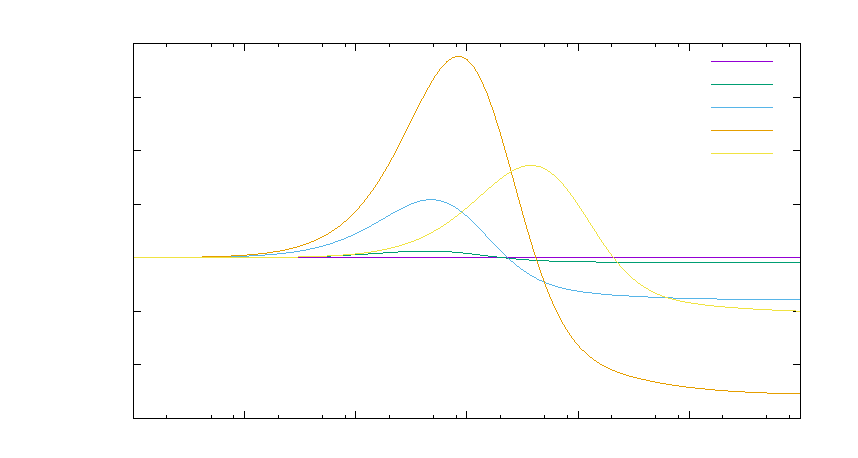
\includegraphics{img/cgBar1L}}%
    \gplfronttext
  \end{picture}%
\endgroup

\end{subfigure}\\%
\begin{subfigure}[t]{\textwidth}
	% GNUPLOT: LaTeX picture with Postscript
\begingroup
  \makeatletter
  \providecommand\color[2][]{%
    \GenericError{(gnuplot) \space\space\space\@spaces}{%
      Package color not loaded in conjunction with
      terminal option `colourtext'%
    }{See the gnuplot documentation for explanation.%
    }{Either use 'blacktext' in gnuplot or load the package
      color.sty in LaTeX.}%
    \renewcommand\color[2][]{}%
  }%
  \providecommand\includegraphics[2][]{%
    \GenericError{(gnuplot) \space\space\space\@spaces}{%
      Package graphicx or graphics not loaded%
    }{See the gnuplot documentation for explanation.%
    }{The gnuplot epslatex terminal needs graphicx.sty or graphics.sty.}%
    \renewcommand\includegraphics[2][]{}%
  }%
  \providecommand\rotatebox[2]{#2}%
  \@ifundefined{ifGPcolor}{%
    \newif\ifGPcolor
    \GPcolorfalse
  }{}%
  \@ifundefined{ifGPblacktext}{%
    \newif\ifGPblacktext
    \GPblacktexttrue
  }{}%
  % define a \g@addto@macro without @ in the name:
  \let\gplgaddtomacro\g@addto@macro
  % define empty templates for all commands taking text:
  \gdef\gplbacktext{}%
  \gdef\gplfronttext{}%
  \makeatother
  \ifGPblacktext
    % no textcolor at all
    \def\colorrgb#1{}%
    \def\colorgray#1{}%
  \else
    % gray or color?
    \ifGPcolor
      \def\colorrgb#1{\color[rgb]{#1}}%
      \def\colorgray#1{\color[gray]{#1}}%
      \expandafter\def\csname LTw\endcsname{\color{white}}%
      \expandafter\def\csname LTb\endcsname{\color{black}}%
      \expandafter\def\csname LTa\endcsname{\color{black}}%
      \expandafter\def\csname LT0\endcsname{\color[rgb]{1,0,0}}%
      \expandafter\def\csname LT1\endcsname{\color[rgb]{0,1,0}}%
      \expandafter\def\csname LT2\endcsname{\color[rgb]{0,0,1}}%
      \expandafter\def\csname LT3\endcsname{\color[rgb]{1,0,1}}%
      \expandafter\def\csname LT4\endcsname{\color[rgb]{0,1,1}}%
      \expandafter\def\csname LT5\endcsname{\color[rgb]{1,1,0}}%
      \expandafter\def\csname LT6\endcsname{\color[rgb]{0,0,0}}%
      \expandafter\def\csname LT7\endcsname{\color[rgb]{1,0.3,0}}%
      \expandafter\def\csname LT8\endcsname{\color[rgb]{0.5,0.5,0.5}}%
    \else
      % gray
      \def\colorrgb#1{\color{black}}%
      \def\colorgray#1{\color[gray]{#1}}%
      \expandafter\def\csname LTw\endcsname{\color{white}}%
      \expandafter\def\csname LTb\endcsname{\color{black}}%
      \expandafter\def\csname LTa\endcsname{\color{black}}%
      \expandafter\def\csname LT0\endcsname{\color{black}}%
      \expandafter\def\csname LT1\endcsname{\color{black}}%
      \expandafter\def\csname LT2\endcsname{\color{black}}%
      \expandafter\def\csname LT3\endcsname{\color{black}}%
      \expandafter\def\csname LT4\endcsname{\color{black}}%
      \expandafter\def\csname LT5\endcsname{\color{black}}%
      \expandafter\def\csname LT6\endcsname{\color{black}}%
      \expandafter\def\csname LT7\endcsname{\color{black}}%
      \expandafter\def\csname LT8\endcsname{\color{black}}%
    \fi
  \fi
    \setlength{\unitlength}{0.0500bp}%
    \ifx\gptboxheight\undefined%
      \newlength{\gptboxheight}%
      \newlength{\gptboxwidth}%
      \newsavebox{\gptboxtext}%
    \fi%
    \setlength{\fboxrule}{0.5pt}%
    \setlength{\fboxsep}{1pt}%
\begin{picture}(7920.00,4082.40)%
    \gplgaddtomacro\gplbacktext{%
      \csname LTb\endcsname%
      \put(990,220){\makebox(0,0)[r]{\strut{} -0.04}}%
      \put(990,734){\makebox(0,0)[r]{\strut{} -0.02}}%
      \put(990,1248){\makebox(0,0)[r]{\strut{} 0.00}}%
      \put(990,1762){\makebox(0,0)[r]{\strut{} 0.02}}%
      \put(990,2276){\makebox(0,0)[r]{\strut{} 0.04}}%
      \put(990,2790){\makebox(0,0)[r]{\strut{} 0.06}}%
      \put(990,3304){\makebox(0,0)[r]{\strut{} 0.08}}%
      \put(990,3818){\makebox(0,0)[r]{\strut{} 0.10}}%
      \put(1122,0){\makebox(0,0){\strut{}$0.001$}}%
      \put(2189,0){\makebox(0,0){\strut{}$0.01$}}%
      \put(3255,0){\makebox(0,0){\strut{}$0.1$}}%
      \put(4322,0){\makebox(0,0){\strut{}$1$}}%
      \put(5389,0){\makebox(0,0){\strut{}$10$}}%
      \put(6455,0){\makebox(0,0){\strut{}$100$}}%
      \put(7522,0){\makebox(0,0){\strut{}$1000$}}%
      \put(1250,3458){\makebox(0,0)[l]{\strut{}(c) $\bar c_{P,g}^{(1)}(\eta)$}}%
    }%
    \gplgaddtomacro\gplfronttext{%
      \csname LTb\endcsname%
      \put(5611,3645){\makebox(0,0)[l]{\strut{}$Q^2=10^{-2}$}}%
      \csname LTb\endcsname%
      \put(5611,3425){\makebox(0,0)[l]{\strut{}$Q^2=10^0$}}%
      \csname LTb\endcsname%
      \put(5611,3205){\makebox(0,0)[l]{\strut{}$Q^2=10^1$}}%
      \csname LTb\endcsname%
      \put(5611,2985){\makebox(0,0)[l]{\strut{}$Q^2=10^2$}}%
      \csname LTb\endcsname%
      \put(5611,2765){\makebox(0,0)[l]{\strut{}$Q^2=10^3$}}%
    }%
    \gplbacktext
    \put(0,0){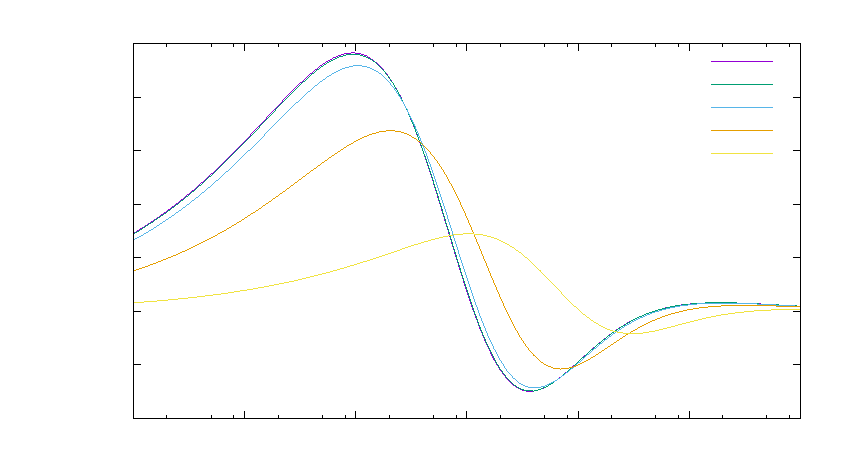
\includegraphics{img/cgBar1P}}%
    \gplfronttext
  \end{picture}%
\endgroup

\end{subfigure}
\caption{next-to-leading order scaling functions $\bar c_{k,g}^{(1)}(\eta,\xi) = \bar c_{k,g}^{R,(1)}(\eta,\xi)+\bar c_{k,g}^{F,(1)}(\eta,\xi)$ plotted as function of $\eta=s/(4m^2)-1$ for different values of $Q^2$ in units of $\si{\GeV^2}$ at $m=\SI{4.75}{\GeV}$ (i.e. different values of $\xi=Q^2/m^2$) and $n_{lf}=4$ }\label{fig:cgBar1}
\end{figure}

\pagebreak
\begin{figure}[ht!]
\centering
\begin{subfigure}[t]{\textwidth}
	% GNUPLOT: LaTeX picture with Postscript
\begingroup
  \makeatletter
  \providecommand\color[2][]{%
    \GenericError{(gnuplot) \space\space\space\@spaces}{%
      Package color not loaded in conjunction with
      terminal option `colourtext'%
    }{See the gnuplot documentation for explanation.%
    }{Either use 'blacktext' in gnuplot or load the package
      color.sty in LaTeX.}%
    \renewcommand\color[2][]{}%
  }%
  \providecommand\includegraphics[2][]{%
    \GenericError{(gnuplot) \space\space\space\@spaces}{%
      Package graphicx or graphics not loaded%
    }{See the gnuplot documentation for explanation.%
    }{The gnuplot epslatex terminal needs graphicx.sty or graphics.sty.}%
    \renewcommand\includegraphics[2][]{}%
  }%
  \providecommand\rotatebox[2]{#2}%
  \@ifundefined{ifGPcolor}{%
    \newif\ifGPcolor
    \GPcolorfalse
  }{}%
  \@ifundefined{ifGPblacktext}{%
    \newif\ifGPblacktext
    \GPblacktexttrue
  }{}%
  % define a \g@addto@macro without @ in the name:
  \let\gplgaddtomacro\g@addto@macro
  % define empty templates for all commands taking text:
  \gdef\gplbacktext{}%
  \gdef\gplfronttext{}%
  \makeatother
  \ifGPblacktext
    % no textcolor at all
    \def\colorrgb#1{}%
    \def\colorgray#1{}%
  \else
    % gray or color?
    \ifGPcolor
      \def\colorrgb#1{\color[rgb]{#1}}%
      \def\colorgray#1{\color[gray]{#1}}%
      \expandafter\def\csname LTw\endcsname{\color{white}}%
      \expandafter\def\csname LTb\endcsname{\color{black}}%
      \expandafter\def\csname LTa\endcsname{\color{black}}%
      \expandafter\def\csname LT0\endcsname{\color[rgb]{1,0,0}}%
      \expandafter\def\csname LT1\endcsname{\color[rgb]{0,1,0}}%
      \expandafter\def\csname LT2\endcsname{\color[rgb]{0,0,1}}%
      \expandafter\def\csname LT3\endcsname{\color[rgb]{1,0,1}}%
      \expandafter\def\csname LT4\endcsname{\color[rgb]{0,1,1}}%
      \expandafter\def\csname LT5\endcsname{\color[rgb]{1,1,0}}%
      \expandafter\def\csname LT6\endcsname{\color[rgb]{0,0,0}}%
      \expandafter\def\csname LT7\endcsname{\color[rgb]{1,0.3,0}}%
      \expandafter\def\csname LT8\endcsname{\color[rgb]{0.5,0.5,0.5}}%
    \else
      % gray
      \def\colorrgb#1{\color{black}}%
      \def\colorgray#1{\color[gray]{#1}}%
      \expandafter\def\csname LTw\endcsname{\color{white}}%
      \expandafter\def\csname LTb\endcsname{\color{black}}%
      \expandafter\def\csname LTa\endcsname{\color{black}}%
      \expandafter\def\csname LT0\endcsname{\color{black}}%
      \expandafter\def\csname LT1\endcsname{\color{black}}%
      \expandafter\def\csname LT2\endcsname{\color{black}}%
      \expandafter\def\csname LT3\endcsname{\color{black}}%
      \expandafter\def\csname LT4\endcsname{\color{black}}%
      \expandafter\def\csname LT5\endcsname{\color{black}}%
      \expandafter\def\csname LT6\endcsname{\color{black}}%
      \expandafter\def\csname LT7\endcsname{\color{black}}%
      \expandafter\def\csname LT8\endcsname{\color{black}}%
    \fi
  \fi
    \setlength{\unitlength}{0.0500bp}%
    \ifx\gptboxheight\undefined%
      \newlength{\gptboxheight}%
      \newlength{\gptboxwidth}%
      \newsavebox{\gptboxtext}%
    \fi%
    \setlength{\fboxrule}{0.5pt}%
    \setlength{\fboxsep}{1pt}%
\begin{picture}(7920.00,4082.40)%
    \gplgaddtomacro\gplbacktext{%
      \csname LTb\endcsname%
      \put(990,220){\makebox(0,0)[r]{\strut{} -0.02}}%
      \put(990,620){\makebox(0,0)[r]{\strut{} 0.00}}%
      \put(990,1020){\makebox(0,0)[r]{\strut{} 0.02}}%
      \put(990,1419){\makebox(0,0)[r]{\strut{} 0.04}}%
      \put(990,1819){\makebox(0,0)[r]{\strut{} 0.06}}%
      \put(990,2219){\makebox(0,0)[r]{\strut{} 0.08}}%
      \put(990,2619){\makebox(0,0)[r]{\strut{} 0.10}}%
      \put(990,3018){\makebox(0,0)[r]{\strut{} 0.12}}%
      \put(990,3418){\makebox(0,0)[r]{\strut{} 0.14}}%
      \put(990,3818){\makebox(0,0)[r]{\strut{} 0.16}}%
      \put(1122,0){\makebox(0,0){\strut{}$0.001$}}%
      \put(2189,0){\makebox(0,0){\strut{}$0.01$}}%
      \put(3255,0){\makebox(0,0){\strut{}$0.1$}}%
      \put(4322,0){\makebox(0,0){\strut{}$1$}}%
      \put(5389,0){\makebox(0,0){\strut{}$10$}}%
      \put(6455,0){\makebox(0,0){\strut{}$100$}}%
      \put(7522,0){\makebox(0,0){\strut{}$1000$}}%
      \put(1250,3458){\makebox(0,0)[l]{\strut{}(a) $c_{T,q}^{(1)}(\eta)$}}%
    }%
    \gplgaddtomacro\gplfronttext{%
      \csname LTb\endcsname%
      \put(1254,2459){\makebox(0,0)[l]{\strut{}$Q^2=10^{-2}$}}%
      \csname LTb\endcsname%
      \put(1254,2239){\makebox(0,0)[l]{\strut{}$Q^2=10^0$}}%
      \csname LTb\endcsname%
      \put(1254,2019){\makebox(0,0)[l]{\strut{}$Q^2=10^1$}}%
      \csname LTb\endcsname%
      \put(1254,1799){\makebox(0,0)[l]{\strut{}$Q^2=10^2$}}%
      \csname LTb\endcsname%
      \put(1254,1579){\makebox(0,0)[l]{\strut{}$Q^2=10^3$}}%
    }%
    \gplbacktext
    \put(0,0){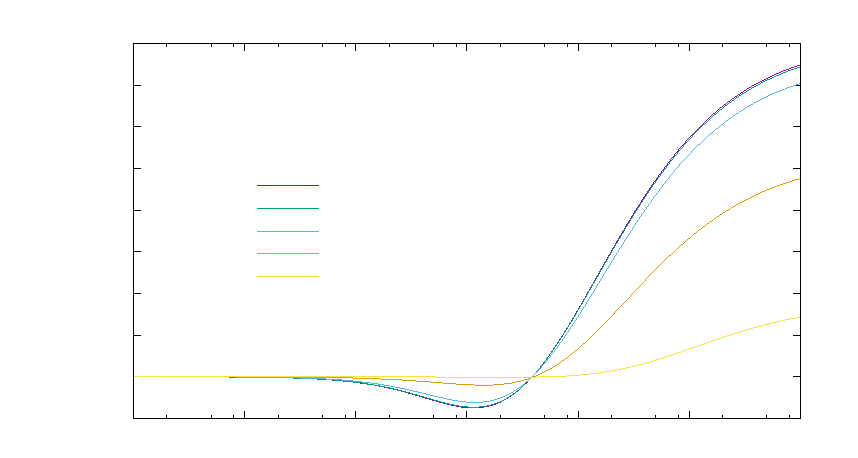
\includegraphics{img/cq1T}}%
    \gplfronttext
  \end{picture}%
\endgroup

\end{subfigure}\\%
\begin{subfigure}[t]{\textwidth}
	% GNUPLOT: LaTeX picture with Postscript
\begingroup
  \makeatletter
  \providecommand\color[2][]{%
    \GenericError{(gnuplot) \space\space\space\@spaces}{%
      Package color not loaded in conjunction with
      terminal option `colourtext'%
    }{See the gnuplot documentation for explanation.%
    }{Either use 'blacktext' in gnuplot or load the package
      color.sty in LaTeX.}%
    \renewcommand\color[2][]{}%
  }%
  \providecommand\includegraphics[2][]{%
    \GenericError{(gnuplot) \space\space\space\@spaces}{%
      Package graphicx or graphics not loaded%
    }{See the gnuplot documentation for explanation.%
    }{The gnuplot epslatex terminal needs graphicx.sty or graphics.sty.}%
    \renewcommand\includegraphics[2][]{}%
  }%
  \providecommand\rotatebox[2]{#2}%
  \@ifundefined{ifGPcolor}{%
    \newif\ifGPcolor
    \GPcolorfalse
  }{}%
  \@ifundefined{ifGPblacktext}{%
    \newif\ifGPblacktext
    \GPblacktexttrue
  }{}%
  % define a \g@addto@macro without @ in the name:
  \let\gplgaddtomacro\g@addto@macro
  % define empty templates for all commands taking text:
  \gdef\gplbacktext{}%
  \gdef\gplfronttext{}%
  \makeatother
  \ifGPblacktext
    % no textcolor at all
    \def\colorrgb#1{}%
    \def\colorgray#1{}%
  \else
    % gray or color?
    \ifGPcolor
      \def\colorrgb#1{\color[rgb]{#1}}%
      \def\colorgray#1{\color[gray]{#1}}%
      \expandafter\def\csname LTw\endcsname{\color{white}}%
      \expandafter\def\csname LTb\endcsname{\color{black}}%
      \expandafter\def\csname LTa\endcsname{\color{black}}%
      \expandafter\def\csname LT0\endcsname{\color[rgb]{1,0,0}}%
      \expandafter\def\csname LT1\endcsname{\color[rgb]{0,1,0}}%
      \expandafter\def\csname LT2\endcsname{\color[rgb]{0,0,1}}%
      \expandafter\def\csname LT3\endcsname{\color[rgb]{1,0,1}}%
      \expandafter\def\csname LT4\endcsname{\color[rgb]{0,1,1}}%
      \expandafter\def\csname LT5\endcsname{\color[rgb]{1,1,0}}%
      \expandafter\def\csname LT6\endcsname{\color[rgb]{0,0,0}}%
      \expandafter\def\csname LT7\endcsname{\color[rgb]{1,0.3,0}}%
      \expandafter\def\csname LT8\endcsname{\color[rgb]{0.5,0.5,0.5}}%
    \else
      % gray
      \def\colorrgb#1{\color{black}}%
      \def\colorgray#1{\color[gray]{#1}}%
      \expandafter\def\csname LTw\endcsname{\color{white}}%
      \expandafter\def\csname LTb\endcsname{\color{black}}%
      \expandafter\def\csname LTa\endcsname{\color{black}}%
      \expandafter\def\csname LT0\endcsname{\color{black}}%
      \expandafter\def\csname LT1\endcsname{\color{black}}%
      \expandafter\def\csname LT2\endcsname{\color{black}}%
      \expandafter\def\csname LT3\endcsname{\color{black}}%
      \expandafter\def\csname LT4\endcsname{\color{black}}%
      \expandafter\def\csname LT5\endcsname{\color{black}}%
      \expandafter\def\csname LT6\endcsname{\color{black}}%
      \expandafter\def\csname LT7\endcsname{\color{black}}%
      \expandafter\def\csname LT8\endcsname{\color{black}}%
    \fi
  \fi
    \setlength{\unitlength}{0.0500bp}%
    \ifx\gptboxheight\undefined%
      \newlength{\gptboxheight}%
      \newlength{\gptboxwidth}%
      \newsavebox{\gptboxtext}%
    \fi%
    \setlength{\fboxrule}{0.5pt}%
    \setlength{\fboxsep}{1pt}%
\begin{picture}(7920.00,4082.40)%
    \gplgaddtomacro\gplbacktext{%
      \csname LTb\endcsname%
      \put(990,220){\makebox(0,0)[r]{\strut{}-0.002}}%
      \put(990,670){\makebox(0,0)[r]{\strut{}0.000}}%
      \put(990,1120){\makebox(0,0)[r]{\strut{}0.002}}%
      \put(990,1569){\makebox(0,0)[r]{\strut{}0.004}}%
      \put(990,2019){\makebox(0,0)[r]{\strut{}0.006}}%
      \put(990,2469){\makebox(0,0)[r]{\strut{}0.008}}%
      \put(990,2919){\makebox(0,0)[r]{\strut{}0.010}}%
      \put(990,3368){\makebox(0,0)[r]{\strut{}0.012}}%
      \put(990,3818){\makebox(0,0)[r]{\strut{}0.014}}%
      \put(1122,0){\makebox(0,0){\strut{}$0.001$}}%
      \put(2189,0){\makebox(0,0){\strut{}$0.01$}}%
      \put(3255,0){\makebox(0,0){\strut{}$0.1$}}%
      \put(4322,0){\makebox(0,0){\strut{}$1$}}%
      \put(5389,0){\makebox(0,0){\strut{}$10$}}%
      \put(6455,0){\makebox(0,0){\strut{}$100$}}%
      \put(7522,0){\makebox(0,0){\strut{}$1000$}}%
      \put(1250,3458){\makebox(0,0)[l]{\strut{}(b) $c_{L,q}^{(1)}(\eta)$}}%
    }%
    \gplgaddtomacro\gplfronttext{%
      \csname LTb\endcsname%
      \put(1254,2459){\makebox(0,0)[l]{\strut{}$Q^2=10^{-2}$}}%
      \csname LTb\endcsname%
      \put(1254,2239){\makebox(0,0)[l]{\strut{}$Q^2=10^0$}}%
      \csname LTb\endcsname%
      \put(1254,2019){\makebox(0,0)[l]{\strut{}$Q^2=10^1$}}%
      \csname LTb\endcsname%
      \put(1254,1799){\makebox(0,0)[l]{\strut{}$Q^2=10^2$}}%
      \csname LTb\endcsname%
      \put(1254,1579){\makebox(0,0)[l]{\strut{}$Q^2=10^3$}}%
    }%
    \gplbacktext
    \put(0,0){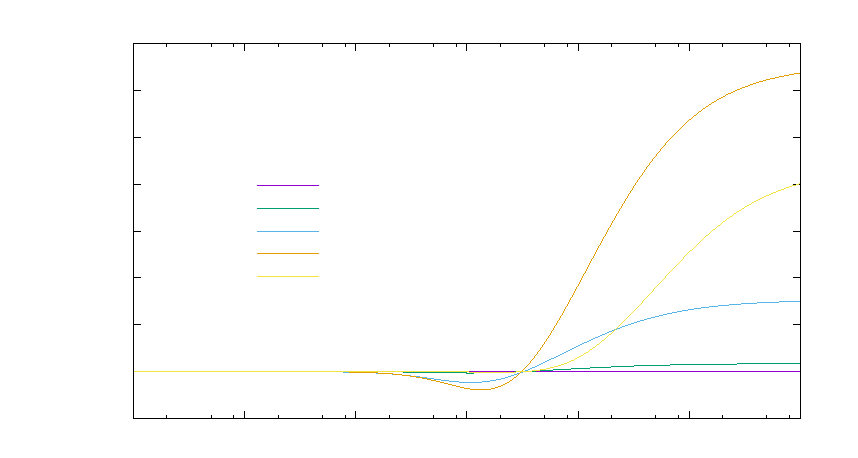
\includegraphics{img/cq1L}}%
    \gplfronttext
  \end{picture}%
\endgroup

\end{subfigure}\\%
\begin{subfigure}[t]{\textwidth}
	% GNUPLOT: LaTeX picture with Postscript
\begingroup
  \makeatletter
  \providecommand\color[2][]{%
    \GenericError{(gnuplot) \space\space\space\@spaces}{%
      Package color not loaded in conjunction with
      terminal option `colourtext'%
    }{See the gnuplot documentation for explanation.%
    }{Either use 'blacktext' in gnuplot or load the package
      color.sty in LaTeX.}%
    \renewcommand\color[2][]{}%
  }%
  \providecommand\includegraphics[2][]{%
    \GenericError{(gnuplot) \space\space\space\@spaces}{%
      Package graphicx or graphics not loaded%
    }{See the gnuplot documentation for explanation.%
    }{The gnuplot epslatex terminal needs graphicx.sty or graphics.sty.}%
    \renewcommand\includegraphics[2][]{}%
  }%
  \providecommand\rotatebox[2]{#2}%
  \@ifundefined{ifGPcolor}{%
    \newif\ifGPcolor
    \GPcolorfalse
  }{}%
  \@ifundefined{ifGPblacktext}{%
    \newif\ifGPblacktext
    \GPblacktexttrue
  }{}%
  % define a \g@addto@macro without @ in the name:
  \let\gplgaddtomacro\g@addto@macro
  % define empty templates for all commands taking text:
  \gdef\gplbacktext{}%
  \gdef\gplfronttext{}%
  \makeatother
  \ifGPblacktext
    % no textcolor at all
    \def\colorrgb#1{}%
    \def\colorgray#1{}%
  \else
    % gray or color?
    \ifGPcolor
      \def\colorrgb#1{\color[rgb]{#1}}%
      \def\colorgray#1{\color[gray]{#1}}%
      \expandafter\def\csname LTw\endcsname{\color{white}}%
      \expandafter\def\csname LTb\endcsname{\color{black}}%
      \expandafter\def\csname LTa\endcsname{\color{black}}%
      \expandafter\def\csname LT0\endcsname{\color[rgb]{1,0,0}}%
      \expandafter\def\csname LT1\endcsname{\color[rgb]{0,1,0}}%
      \expandafter\def\csname LT2\endcsname{\color[rgb]{0,0,1}}%
      \expandafter\def\csname LT3\endcsname{\color[rgb]{1,0,1}}%
      \expandafter\def\csname LT4\endcsname{\color[rgb]{0,1,1}}%
      \expandafter\def\csname LT5\endcsname{\color[rgb]{1,1,0}}%
      \expandafter\def\csname LT6\endcsname{\color[rgb]{0,0,0}}%
      \expandafter\def\csname LT7\endcsname{\color[rgb]{1,0.3,0}}%
      \expandafter\def\csname LT8\endcsname{\color[rgb]{0.5,0.5,0.5}}%
    \else
      % gray
      \def\colorrgb#1{\color{black}}%
      \def\colorgray#1{\color[gray]{#1}}%
      \expandafter\def\csname LTw\endcsname{\color{white}}%
      \expandafter\def\csname LTb\endcsname{\color{black}}%
      \expandafter\def\csname LTa\endcsname{\color{black}}%
      \expandafter\def\csname LT0\endcsname{\color{black}}%
      \expandafter\def\csname LT1\endcsname{\color{black}}%
      \expandafter\def\csname LT2\endcsname{\color{black}}%
      \expandafter\def\csname LT3\endcsname{\color{black}}%
      \expandafter\def\csname LT4\endcsname{\color{black}}%
      \expandafter\def\csname LT5\endcsname{\color{black}}%
      \expandafter\def\csname LT6\endcsname{\color{black}}%
      \expandafter\def\csname LT7\endcsname{\color{black}}%
      \expandafter\def\csname LT8\endcsname{\color{black}}%
    \fi
  \fi
    \setlength{\unitlength}{0.0500bp}%
    \ifx\gptboxheight\undefined%
      \newlength{\gptboxheight}%
      \newlength{\gptboxwidth}%
      \newsavebox{\gptboxtext}%
    \fi%
    \setlength{\fboxrule}{0.5pt}%
    \setlength{\fboxsep}{1pt}%
\begin{picture}(7920.00,4082.40)%
    \gplgaddtomacro\gplbacktext{%
      \csname LTb\endcsname%
      \put(990,220){\makebox(0,0)[r]{\strut{}-0.010}}%
      \put(990,620){\makebox(0,0)[r]{\strut{}-0.008}}%
      \put(990,1020){\makebox(0,0)[r]{\strut{}-0.006}}%
      \put(990,1419){\makebox(0,0)[r]{\strut{}-0.004}}%
      \put(990,1819){\makebox(0,0)[r]{\strut{}-0.002}}%
      \put(990,2219){\makebox(0,0)[r]{\strut{}0.000}}%
      \put(990,2619){\makebox(0,0)[r]{\strut{}0.002}}%
      \put(990,3018){\makebox(0,0)[r]{\strut{}0.004}}%
      \put(990,3418){\makebox(0,0)[r]{\strut{}0.006}}%
      \put(990,3818){\makebox(0,0)[r]{\strut{}0.008}}%
      \put(1122,0){\makebox(0,0){\strut{}$0.001$}}%
      \put(2189,0){\makebox(0,0){\strut{}$0.01$}}%
      \put(3255,0){\makebox(0,0){\strut{}$0.1$}}%
      \put(4322,0){\makebox(0,0){\strut{}$1$}}%
      \put(5389,0){\makebox(0,0){\strut{}$10$}}%
      \put(6455,0){\makebox(0,0){\strut{}$100$}}%
      \put(7522,0){\makebox(0,0){\strut{}$1000$}}%
      \put(1250,3458){\makebox(0,0)[l]{\strut{}(c) $c_{P,q}^{(1)}(\eta)$}}%
    }%
    \gplgaddtomacro\gplfronttext{%
      \csname LTb\endcsname%
      \put(1254,1273){\makebox(0,0)[l]{\strut{}$Q^2=10^{-2}$}}%
      \csname LTb\endcsname%
      \put(1254,1053){\makebox(0,0)[l]{\strut{}$Q^2=10^0$}}%
      \csname LTb\endcsname%
      \put(1254,833){\makebox(0,0)[l]{\strut{}$Q^2=10^1$}}%
      \csname LTb\endcsname%
      \put(1254,613){\makebox(0,0)[l]{\strut{}$Q^2=10^2$}}%
      \csname LTb\endcsname%
      \put(1254,393){\makebox(0,0)[l]{\strut{}$Q^2=10^3$}}%
    }%
    \gplbacktext
    \put(0,0){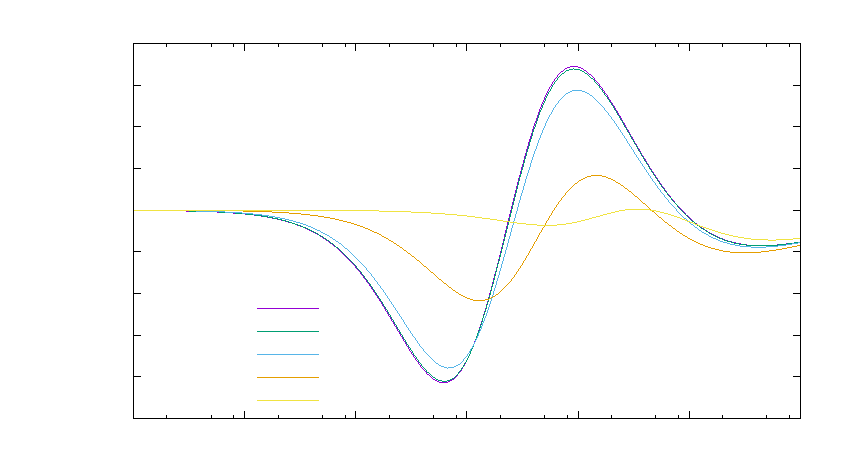
\includegraphics{img/cq1P}}%
    \gplfronttext
  \end{picture}%
\endgroup

\end{subfigure}
\caption{next-to-leading order scaling functions $c_{k,q}^{(1)}(\eta,\xi)$ plotted as function of $\eta=s/(4m^2)-1$ for different values of $Q^2$ in units of $\si{\GeV^2}$ at $m=\SI{4.75}{\GeV}$ (i.e. different values of $\xi=Q^2/m^2$). Note that \cite[Fig. 9 (b)]{Laenen1993162} is wrong. }\label{fig:cq1}
\end{figure}

\pagebreak
\begin{figure}[ht!]
\centering
\begin{subfigure}[t]{\textwidth}
	% GNUPLOT: LaTeX picture with Postscript
\begingroup
  \makeatletter
  \providecommand\color[2][]{%
    \GenericError{(gnuplot) \space\space\space\@spaces}{%
      Package color not loaded in conjunction with
      terminal option `colourtext'%
    }{See the gnuplot documentation for explanation.%
    }{Either use 'blacktext' in gnuplot or load the package
      color.sty in LaTeX.}%
    \renewcommand\color[2][]{}%
  }%
  \providecommand\includegraphics[2][]{%
    \GenericError{(gnuplot) \space\space\space\@spaces}{%
      Package graphicx or graphics not loaded%
    }{See the gnuplot documentation for explanation.%
    }{The gnuplot epslatex terminal needs graphicx.sty or graphics.sty.}%
    \renewcommand\includegraphics[2][]{}%
  }%
  \providecommand\rotatebox[2]{#2}%
  \@ifundefined{ifGPcolor}{%
    \newif\ifGPcolor
    \GPcolorfalse
  }{}%
  \@ifundefined{ifGPblacktext}{%
    \newif\ifGPblacktext
    \GPblacktexttrue
  }{}%
  % define a \g@addto@macro without @ in the name:
  \let\gplgaddtomacro\g@addto@macro
  % define empty templates for all commands taking text:
  \gdef\gplbacktext{}%
  \gdef\gplfronttext{}%
  \makeatother
  \ifGPblacktext
    % no textcolor at all
    \def\colorrgb#1{}%
    \def\colorgray#1{}%
  \else
    % gray or color?
    \ifGPcolor
      \def\colorrgb#1{\color[rgb]{#1}}%
      \def\colorgray#1{\color[gray]{#1}}%
      \expandafter\def\csname LTw\endcsname{\color{white}}%
      \expandafter\def\csname LTb\endcsname{\color{black}}%
      \expandafter\def\csname LTa\endcsname{\color{black}}%
      \expandafter\def\csname LT0\endcsname{\color[rgb]{1,0,0}}%
      \expandafter\def\csname LT1\endcsname{\color[rgb]{0,1,0}}%
      \expandafter\def\csname LT2\endcsname{\color[rgb]{0,0,1}}%
      \expandafter\def\csname LT3\endcsname{\color[rgb]{1,0,1}}%
      \expandafter\def\csname LT4\endcsname{\color[rgb]{0,1,1}}%
      \expandafter\def\csname LT5\endcsname{\color[rgb]{1,1,0}}%
      \expandafter\def\csname LT6\endcsname{\color[rgb]{0,0,0}}%
      \expandafter\def\csname LT7\endcsname{\color[rgb]{1,0.3,0}}%
      \expandafter\def\csname LT8\endcsname{\color[rgb]{0.5,0.5,0.5}}%
    \else
      % gray
      \def\colorrgb#1{\color{black}}%
      \def\colorgray#1{\color[gray]{#1}}%
      \expandafter\def\csname LTw\endcsname{\color{white}}%
      \expandafter\def\csname LTb\endcsname{\color{black}}%
      \expandafter\def\csname LTa\endcsname{\color{black}}%
      \expandafter\def\csname LT0\endcsname{\color{black}}%
      \expandafter\def\csname LT1\endcsname{\color{black}}%
      \expandafter\def\csname LT2\endcsname{\color{black}}%
      \expandafter\def\csname LT3\endcsname{\color{black}}%
      \expandafter\def\csname LT4\endcsname{\color{black}}%
      \expandafter\def\csname LT5\endcsname{\color{black}}%
      \expandafter\def\csname LT6\endcsname{\color{black}}%
      \expandafter\def\csname LT7\endcsname{\color{black}}%
      \expandafter\def\csname LT8\endcsname{\color{black}}%
    \fi
  \fi
    \setlength{\unitlength}{0.0500bp}%
    \ifx\gptboxheight\undefined%
      \newlength{\gptboxheight}%
      \newlength{\gptboxwidth}%
      \newsavebox{\gptboxtext}%
    \fi%
    \setlength{\fboxrule}{0.5pt}%
    \setlength{\fboxsep}{1pt}%
\begin{picture}(7920.00,4082.40)%
    \gplgaddtomacro\gplbacktext{%
      \csname LTb\endcsname%
      \put(990,220){\makebox(0,0)[r]{\strut{} -0.09}}%
      \put(990,620){\makebox(0,0)[r]{\strut{} -0.08}}%
      \put(990,1020){\makebox(0,0)[r]{\strut{} -0.07}}%
      \put(990,1419){\makebox(0,0)[r]{\strut{} -0.06}}%
      \put(990,1819){\makebox(0,0)[r]{\strut{} -0.05}}%
      \put(990,2219){\makebox(0,0)[r]{\strut{} -0.04}}%
      \put(990,2619){\makebox(0,0)[r]{\strut{} -0.03}}%
      \put(990,3018){\makebox(0,0)[r]{\strut{} -0.02}}%
      \put(990,3418){\makebox(0,0)[r]{\strut{} -0.01}}%
      \put(990,3818){\makebox(0,0)[r]{\strut{} 0.00}}%
      \put(1122,0){\makebox(0,0){\strut{}$0.001$}}%
      \put(2189,0){\makebox(0,0){\strut{}$0.01$}}%
      \put(3255,0){\makebox(0,0){\strut{}$0.1$}}%
      \put(4322,0){\makebox(0,0){\strut{}$1$}}%
      \put(5389,0){\makebox(0,0){\strut{}$10$}}%
      \put(6455,0){\makebox(0,0){\strut{}$100$}}%
      \put(7522,0){\makebox(0,0){\strut{}$1000$}}%
      \put(1250,3458){\makebox(0,0)[l]{\strut{}(a) $\bar c_{T,q}^{F,(1)}(\eta)$}}%
    }%
    \gplgaddtomacro\gplfronttext{%
      \csname LTb\endcsname%
      \put(1254,1273){\makebox(0,0)[l]{\strut{}$Q^2=10^{-2}$}}%
      \csname LTb\endcsname%
      \put(1254,1053){\makebox(0,0)[l]{\strut{}$Q^2=10^0$}}%
      \csname LTb\endcsname%
      \put(1254,833){\makebox(0,0)[l]{\strut{}$Q^2=10^1$}}%
      \csname LTb\endcsname%
      \put(1254,613){\makebox(0,0)[l]{\strut{}$Q^2=10^2$}}%
      \csname LTb\endcsname%
      \put(1254,393){\makebox(0,0)[l]{\strut{}$Q^2=10^3$}}%
    }%
    \gplbacktext
    \put(0,0){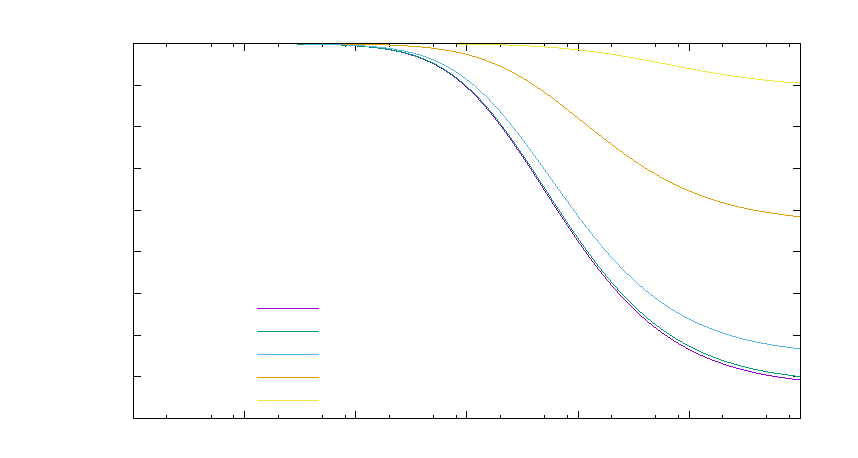
\includegraphics{img/cqBarF1T}}%
    \gplfronttext
  \end{picture}%
\endgroup

\end{subfigure}\\%
\begin{subfigure}[t]{\textwidth}
	% GNUPLOT: LaTeX picture with Postscript
\begingroup
  \makeatletter
  \providecommand\color[2][]{%
    \GenericError{(gnuplot) \space\space\space\@spaces}{%
      Package color not loaded in conjunction with
      terminal option `colourtext'%
    }{See the gnuplot documentation for explanation.%
    }{Either use 'blacktext' in gnuplot or load the package
      color.sty in LaTeX.}%
    \renewcommand\color[2][]{}%
  }%
  \providecommand\includegraphics[2][]{%
    \GenericError{(gnuplot) \space\space\space\@spaces}{%
      Package graphicx or graphics not loaded%
    }{See the gnuplot documentation for explanation.%
    }{The gnuplot epslatex terminal needs graphicx.sty or graphics.sty.}%
    \renewcommand\includegraphics[2][]{}%
  }%
  \providecommand\rotatebox[2]{#2}%
  \@ifundefined{ifGPcolor}{%
    \newif\ifGPcolor
    \GPcolorfalse
  }{}%
  \@ifundefined{ifGPblacktext}{%
    \newif\ifGPblacktext
    \GPblacktexttrue
  }{}%
  % define a \g@addto@macro without @ in the name:
  \let\gplgaddtomacro\g@addto@macro
  % define empty templates for all commands taking text:
  \gdef\gplbacktext{}%
  \gdef\gplfronttext{}%
  \makeatother
  \ifGPblacktext
    % no textcolor at all
    \def\colorrgb#1{}%
    \def\colorgray#1{}%
  \else
    % gray or color?
    \ifGPcolor
      \def\colorrgb#1{\color[rgb]{#1}}%
      \def\colorgray#1{\color[gray]{#1}}%
      \expandafter\def\csname LTw\endcsname{\color{white}}%
      \expandafter\def\csname LTb\endcsname{\color{black}}%
      \expandafter\def\csname LTa\endcsname{\color{black}}%
      \expandafter\def\csname LT0\endcsname{\color[rgb]{1,0,0}}%
      \expandafter\def\csname LT1\endcsname{\color[rgb]{0,1,0}}%
      \expandafter\def\csname LT2\endcsname{\color[rgb]{0,0,1}}%
      \expandafter\def\csname LT3\endcsname{\color[rgb]{1,0,1}}%
      \expandafter\def\csname LT4\endcsname{\color[rgb]{0,1,1}}%
      \expandafter\def\csname LT5\endcsname{\color[rgb]{1,1,0}}%
      \expandafter\def\csname LT6\endcsname{\color[rgb]{0,0,0}}%
      \expandafter\def\csname LT7\endcsname{\color[rgb]{1,0.3,0}}%
      \expandafter\def\csname LT8\endcsname{\color[rgb]{0.5,0.5,0.5}}%
    \else
      % gray
      \def\colorrgb#1{\color{black}}%
      \def\colorgray#1{\color[gray]{#1}}%
      \expandafter\def\csname LTw\endcsname{\color{white}}%
      \expandafter\def\csname LTb\endcsname{\color{black}}%
      \expandafter\def\csname LTa\endcsname{\color{black}}%
      \expandafter\def\csname LT0\endcsname{\color{black}}%
      \expandafter\def\csname LT1\endcsname{\color{black}}%
      \expandafter\def\csname LT2\endcsname{\color{black}}%
      \expandafter\def\csname LT3\endcsname{\color{black}}%
      \expandafter\def\csname LT4\endcsname{\color{black}}%
      \expandafter\def\csname LT5\endcsname{\color{black}}%
      \expandafter\def\csname LT6\endcsname{\color{black}}%
      \expandafter\def\csname LT7\endcsname{\color{black}}%
      \expandafter\def\csname LT8\endcsname{\color{black}}%
    \fi
  \fi
    \setlength{\unitlength}{0.0500bp}%
    \ifx\gptboxheight\undefined%
      \newlength{\gptboxheight}%
      \newlength{\gptboxwidth}%
      \newsavebox{\gptboxtext}%
    \fi%
    \setlength{\fboxrule}{0.5pt}%
    \setlength{\fboxsep}{1pt}%
\begin{picture}(7920.00,4082.40)%
    \gplgaddtomacro\gplbacktext{%
      \csname LTb\endcsname%
      \put(990,220){\makebox(0,0)[r]{\strut{}-0.006}}%
      \put(990,820){\makebox(0,0)[r]{\strut{}-0.005}}%
      \put(990,1419){\makebox(0,0)[r]{\strut{}-0.004}}%
      \put(990,2019){\makebox(0,0)[r]{\strut{}-0.003}}%
      \put(990,2619){\makebox(0,0)[r]{\strut{}-0.002}}%
      \put(990,3218){\makebox(0,0)[r]{\strut{}-0.001}}%
      \put(990,3818){\makebox(0,0)[r]{\strut{}0.000}}%
      \put(1122,0){\makebox(0,0){\strut{}$0.001$}}%
      \put(2189,0){\makebox(0,0){\strut{}$0.01$}}%
      \put(3255,0){\makebox(0,0){\strut{}$0.1$}}%
      \put(4322,0){\makebox(0,0){\strut{}$1$}}%
      \put(5389,0){\makebox(0,0){\strut{}$10$}}%
      \put(6455,0){\makebox(0,0){\strut{}$100$}}%
      \put(7522,0){\makebox(0,0){\strut{}$1000$}}%
      \put(1250,3458){\makebox(0,0)[l]{\strut{}(b) $\bar c_{L,q}^{F,(1)}(\eta)$}}%
    }%
    \gplgaddtomacro\gplfronttext{%
      \csname LTb\endcsname%
      \put(1254,1273){\makebox(0,0)[l]{\strut{}$Q^2=10^{-2}$}}%
      \csname LTb\endcsname%
      \put(1254,1053){\makebox(0,0)[l]{\strut{}$Q^2=10^0$}}%
      \csname LTb\endcsname%
      \put(1254,833){\makebox(0,0)[l]{\strut{}$Q^2=10^1$}}%
      \csname LTb\endcsname%
      \put(1254,613){\makebox(0,0)[l]{\strut{}$Q^2=10^2$}}%
      \csname LTb\endcsname%
      \put(1254,393){\makebox(0,0)[l]{\strut{}$Q^2=10^3$}}%
    }%
    \gplbacktext
    \put(0,0){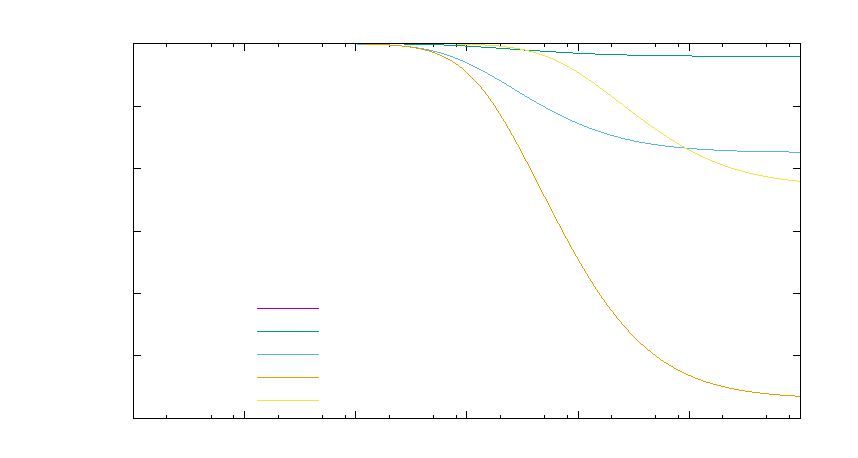
\includegraphics{img/cqBarF1L}}%
    \gplfronttext
  \end{picture}%
\endgroup

\end{subfigure}\\%
\begin{subfigure}[t]{\textwidth}
	% GNUPLOT: LaTeX picture with Postscript
\begingroup
  \makeatletter
  \providecommand\color[2][]{%
    \GenericError{(gnuplot) \space\space\space\@spaces}{%
      Package color not loaded in conjunction with
      terminal option `colourtext'%
    }{See the gnuplot documentation for explanation.%
    }{Either use 'blacktext' in gnuplot or load the package
      color.sty in LaTeX.}%
    \renewcommand\color[2][]{}%
  }%
  \providecommand\includegraphics[2][]{%
    \GenericError{(gnuplot) \space\space\space\@spaces}{%
      Package graphicx or graphics not loaded%
    }{See the gnuplot documentation for explanation.%
    }{The gnuplot epslatex terminal needs graphicx.sty or graphics.sty.}%
    \renewcommand\includegraphics[2][]{}%
  }%
  \providecommand\rotatebox[2]{#2}%
  \@ifundefined{ifGPcolor}{%
    \newif\ifGPcolor
    \GPcolorfalse
  }{}%
  \@ifundefined{ifGPblacktext}{%
    \newif\ifGPblacktext
    \GPblacktexttrue
  }{}%
  % define a \g@addto@macro without @ in the name:
  \let\gplgaddtomacro\g@addto@macro
  % define empty templates for all commands taking text:
  \gdef\gplbacktext{}%
  \gdef\gplfronttext{}%
  \makeatother
  \ifGPblacktext
    % no textcolor at all
    \def\colorrgb#1{}%
    \def\colorgray#1{}%
  \else
    % gray or color?
    \ifGPcolor
      \def\colorrgb#1{\color[rgb]{#1}}%
      \def\colorgray#1{\color[gray]{#1}}%
      \expandafter\def\csname LTw\endcsname{\color{white}}%
      \expandafter\def\csname LTb\endcsname{\color{black}}%
      \expandafter\def\csname LTa\endcsname{\color{black}}%
      \expandafter\def\csname LT0\endcsname{\color[rgb]{1,0,0}}%
      \expandafter\def\csname LT1\endcsname{\color[rgb]{0,1,0}}%
      \expandafter\def\csname LT2\endcsname{\color[rgb]{0,0,1}}%
      \expandafter\def\csname LT3\endcsname{\color[rgb]{1,0,1}}%
      \expandafter\def\csname LT4\endcsname{\color[rgb]{0,1,1}}%
      \expandafter\def\csname LT5\endcsname{\color[rgb]{1,1,0}}%
      \expandafter\def\csname LT6\endcsname{\color[rgb]{0,0,0}}%
      \expandafter\def\csname LT7\endcsname{\color[rgb]{1,0.3,0}}%
      \expandafter\def\csname LT8\endcsname{\color[rgb]{0.5,0.5,0.5}}%
    \else
      % gray
      \def\colorrgb#1{\color{black}}%
      \def\colorgray#1{\color[gray]{#1}}%
      \expandafter\def\csname LTw\endcsname{\color{white}}%
      \expandafter\def\csname LTb\endcsname{\color{black}}%
      \expandafter\def\csname LTa\endcsname{\color{black}}%
      \expandafter\def\csname LT0\endcsname{\color{black}}%
      \expandafter\def\csname LT1\endcsname{\color{black}}%
      \expandafter\def\csname LT2\endcsname{\color{black}}%
      \expandafter\def\csname LT3\endcsname{\color{black}}%
      \expandafter\def\csname LT4\endcsname{\color{black}}%
      \expandafter\def\csname LT5\endcsname{\color{black}}%
      \expandafter\def\csname LT6\endcsname{\color{black}}%
      \expandafter\def\csname LT7\endcsname{\color{black}}%
      \expandafter\def\csname LT8\endcsname{\color{black}}%
    \fi
  \fi
    \setlength{\unitlength}{0.0500bp}%
    \ifx\gptboxheight\undefined%
      \newlength{\gptboxheight}%
      \newlength{\gptboxwidth}%
      \newsavebox{\gptboxtext}%
    \fi%
    \setlength{\fboxrule}{0.5pt}%
    \setlength{\fboxsep}{1pt}%
\begin{picture}(7920.00,4082.40)%
    \gplgaddtomacro\gplbacktext{%
      \csname LTb\endcsname%
      \put(990,220){\makebox(0,0)[r]{\strut{}-0.005}}%
      \put(990,734){\makebox(0,0)[r]{\strut{}-0.004}}%
      \put(990,1248){\makebox(0,0)[r]{\strut{}-0.003}}%
      \put(990,1762){\makebox(0,0)[r]{\strut{}-0.002}}%
      \put(990,2276){\makebox(0,0)[r]{\strut{}-0.001}}%
      \put(990,2790){\makebox(0,0)[r]{\strut{}0.000}}%
      \put(990,3304){\makebox(0,0)[r]{\strut{}0.001}}%
      \put(990,3818){\makebox(0,0)[r]{\strut{}0.002}}%
      \put(1122,0){\makebox(0,0){\strut{}$0.001$}}%
      \put(2189,0){\makebox(0,0){\strut{}$0.01$}}%
      \put(3255,0){\makebox(0,0){\strut{}$0.1$}}%
      \put(4322,0){\makebox(0,0){\strut{}$1$}}%
      \put(5389,0){\makebox(0,0){\strut{}$10$}}%
      \put(6455,0){\makebox(0,0){\strut{}$100$}}%
      \put(7522,0){\makebox(0,0){\strut{}$1000$}}%
      \put(1250,3458){\makebox(0,0)[l]{\strut{}(c) $\bar c_{P,q}^{F,(1)}(\eta)$}}%
    }%
    \gplgaddtomacro\gplfronttext{%
      \csname LTb\endcsname%
      \put(1254,1273){\makebox(0,0)[l]{\strut{}$Q^2=10^{-2}$}}%
      \csname LTb\endcsname%
      \put(1254,1053){\makebox(0,0)[l]{\strut{}$Q^2=10^0$}}%
      \csname LTb\endcsname%
      \put(1254,833){\makebox(0,0)[l]{\strut{}$Q^2=10^1$}}%
      \csname LTb\endcsname%
      \put(1254,613){\makebox(0,0)[l]{\strut{}$Q^2=10^2$}}%
      \csname LTb\endcsname%
      \put(1254,393){\makebox(0,0)[l]{\strut{}$Q^2=10^3$}}%
    }%
    \gplbacktext
    \put(0,0){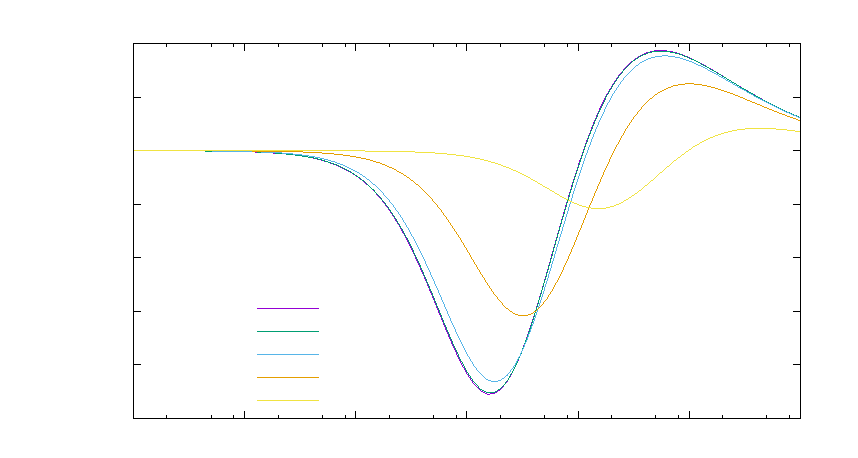
\includegraphics{img/cqBarF1P}}%
    \gplfronttext
  \end{picture}%
\endgroup

\end{subfigure}
\caption{next-to-leading order scaling functions $\bar c_{k,q}^{F,(1)}(\eta,\xi)$ plotted as function of $\eta=s/(4m^2)-1$ for different values of $Q^2$ in units of $\si{\GeV^2}$ at $m=\SI{4.75}{\GeV}$ (i.e. different values of $\xi=Q^2/m^2$)}\label{fig:cqBarF1}
\end{figure}

\pagebreak
\begin{figure}[ht!]
\centering
\begin{subfigure}[t]{\textwidth}
	% GNUPLOT: LaTeX picture with Postscript
\begingroup
  \makeatletter
  \providecommand\color[2][]{%
    \GenericError{(gnuplot) \space\space\space\@spaces}{%
      Package color not loaded in conjunction with
      terminal option `colourtext'%
    }{See the gnuplot documentation for explanation.%
    }{Either use 'blacktext' in gnuplot or load the package
      color.sty in LaTeX.}%
    \renewcommand\color[2][]{}%
  }%
  \providecommand\includegraphics[2][]{%
    \GenericError{(gnuplot) \space\space\space\@spaces}{%
      Package graphicx or graphics not loaded%
    }{See the gnuplot documentation for explanation.%
    }{The gnuplot epslatex terminal needs graphicx.sty or graphics.sty.}%
    \renewcommand\includegraphics[2][]{}%
  }%
  \providecommand\rotatebox[2]{#2}%
  \@ifundefined{ifGPcolor}{%
    \newif\ifGPcolor
    \GPcolorfalse
  }{}%
  \@ifundefined{ifGPblacktext}{%
    \newif\ifGPblacktext
    \GPblacktexttrue
  }{}%
  % define a \g@addto@macro without @ in the name:
  \let\gplgaddtomacro\g@addto@macro
  % define empty templates for all commands taking text:
  \gdef\gplbacktext{}%
  \gdef\gplfronttext{}%
  \makeatother
  \ifGPblacktext
    % no textcolor at all
    \def\colorrgb#1{}%
    \def\colorgray#1{}%
  \else
    % gray or color?
    \ifGPcolor
      \def\colorrgb#1{\color[rgb]{#1}}%
      \def\colorgray#1{\color[gray]{#1}}%
      \expandafter\def\csname LTw\endcsname{\color{white}}%
      \expandafter\def\csname LTb\endcsname{\color{black}}%
      \expandafter\def\csname LTa\endcsname{\color{black}}%
      \expandafter\def\csname LT0\endcsname{\color[rgb]{1,0,0}}%
      \expandafter\def\csname LT1\endcsname{\color[rgb]{0,1,0}}%
      \expandafter\def\csname LT2\endcsname{\color[rgb]{0,0,1}}%
      \expandafter\def\csname LT3\endcsname{\color[rgb]{1,0,1}}%
      \expandafter\def\csname LT4\endcsname{\color[rgb]{0,1,1}}%
      \expandafter\def\csname LT5\endcsname{\color[rgb]{1,1,0}}%
      \expandafter\def\csname LT6\endcsname{\color[rgb]{0,0,0}}%
      \expandafter\def\csname LT7\endcsname{\color[rgb]{1,0.3,0}}%
      \expandafter\def\csname LT8\endcsname{\color[rgb]{0.5,0.5,0.5}}%
    \else
      % gray
      \def\colorrgb#1{\color{black}}%
      \def\colorgray#1{\color[gray]{#1}}%
      \expandafter\def\csname LTw\endcsname{\color{white}}%
      \expandafter\def\csname LTb\endcsname{\color{black}}%
      \expandafter\def\csname LTa\endcsname{\color{black}}%
      \expandafter\def\csname LT0\endcsname{\color{black}}%
      \expandafter\def\csname LT1\endcsname{\color{black}}%
      \expandafter\def\csname LT2\endcsname{\color{black}}%
      \expandafter\def\csname LT3\endcsname{\color{black}}%
      \expandafter\def\csname LT4\endcsname{\color{black}}%
      \expandafter\def\csname LT5\endcsname{\color{black}}%
      \expandafter\def\csname LT6\endcsname{\color{black}}%
      \expandafter\def\csname LT7\endcsname{\color{black}}%
      \expandafter\def\csname LT8\endcsname{\color{black}}%
    \fi
  \fi
    \setlength{\unitlength}{0.0500bp}%
    \ifx\gptboxheight\undefined%
      \newlength{\gptboxheight}%
      \newlength{\gptboxwidth}%
      \newsavebox{\gptboxtext}%
    \fi%
    \setlength{\fboxrule}{0.5pt}%
    \setlength{\fboxsep}{1pt}%
\begin{picture}(7920.00,4082.40)%
    \gplgaddtomacro\gplbacktext{%
      \csname LTb\endcsname%
      \put(990,220){\makebox(0,0)[r]{\strut{} 0.000}}%
      \put(990,670){\makebox(0,0)[r]{\strut{} 0.002}}%
      \put(990,1120){\makebox(0,0)[r]{\strut{} 0.004}}%
      \put(990,1569){\makebox(0,0)[r]{\strut{} 0.006}}%
      \put(990,2019){\makebox(0,0)[r]{\strut{} 0.008}}%
      \put(990,2469){\makebox(0,0)[r]{\strut{} 0.010}}%
      \put(990,2919){\makebox(0,0)[r]{\strut{} 0.012}}%
      \put(990,3368){\makebox(0,0)[r]{\strut{} 0.014}}%
      \put(990,3818){\makebox(0,0)[r]{\strut{} 0.016}}%
      \put(1122,0){\makebox(0,0){\strut{}$0.001$}}%
      \put(2189,0){\makebox(0,0){\strut{}$0.01$}}%
      \put(3255,0){\makebox(0,0){\strut{}$0.1$}}%
      \put(4322,0){\makebox(0,0){\strut{}$1$}}%
      \put(5389,0){\makebox(0,0){\strut{}$10$}}%
      \put(6455,0){\makebox(0,0){\strut{}$100$}}%
      \put(7522,0){\makebox(0,0){\strut{}$1000$}}%
      \put(1250,3458){\makebox(0,0)[l]{\strut{}(a) $d_{T,q}^{(1)}(\eta)$}}%
    }%
    \gplgaddtomacro\gplfronttext{%
      \csname LTb\endcsname%
      \put(1254,2459){\makebox(0,0)[l]{\strut{}$Q^2=10^{-2}$}}%
      \csname LTb\endcsname%
      \put(1254,2239){\makebox(0,0)[l]{\strut{}$Q^2=10^0$}}%
      \csname LTb\endcsname%
      \put(1254,2019){\makebox(0,0)[l]{\strut{}$Q^2=10^1$}}%
      \csname LTb\endcsname%
      \put(1254,1799){\makebox(0,0)[l]{\strut{}$Q^2=10^2$}}%
      \csname LTb\endcsname%
      \put(1254,1579){\makebox(0,0)[l]{\strut{}$Q^2=10^3$}}%
    }%
    \gplbacktext
    \put(0,0){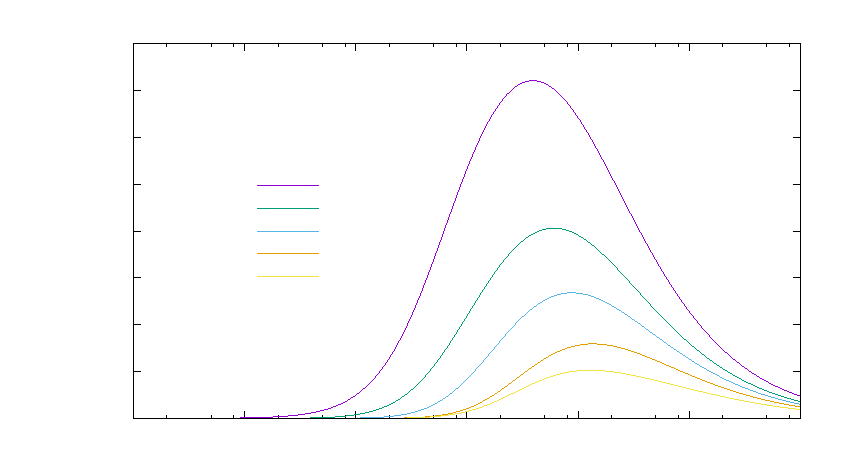
\includegraphics{img/dq1T}}%
    \gplfronttext
  \end{picture}%
\endgroup

\end{subfigure}\\%
\begin{subfigure}[t]{\textwidth}
	% GNUPLOT: LaTeX picture with Postscript
\begingroup
  \makeatletter
  \providecommand\color[2][]{%
    \GenericError{(gnuplot) \space\space\space\@spaces}{%
      Package color not loaded in conjunction with
      terminal option `colourtext'%
    }{See the gnuplot documentation for explanation.%
    }{Either use 'blacktext' in gnuplot or load the package
      color.sty in LaTeX.}%
    \renewcommand\color[2][]{}%
  }%
  \providecommand\includegraphics[2][]{%
    \GenericError{(gnuplot) \space\space\space\@spaces}{%
      Package graphicx or graphics not loaded%
    }{See the gnuplot documentation for explanation.%
    }{The gnuplot epslatex terminal needs graphicx.sty or graphics.sty.}%
    \renewcommand\includegraphics[2][]{}%
  }%
  \providecommand\rotatebox[2]{#2}%
  \@ifundefined{ifGPcolor}{%
    \newif\ifGPcolor
    \GPcolorfalse
  }{}%
  \@ifundefined{ifGPblacktext}{%
    \newif\ifGPblacktext
    \GPblacktexttrue
  }{}%
  % define a \g@addto@macro without @ in the name:
  \let\gplgaddtomacro\g@addto@macro
  % define empty templates for all commands taking text:
  \gdef\gplbacktext{}%
  \gdef\gplfronttext{}%
  \makeatother
  \ifGPblacktext
    % no textcolor at all
    \def\colorrgb#1{}%
    \def\colorgray#1{}%
  \else
    % gray or color?
    \ifGPcolor
      \def\colorrgb#1{\color[rgb]{#1}}%
      \def\colorgray#1{\color[gray]{#1}}%
      \expandafter\def\csname LTw\endcsname{\color{white}}%
      \expandafter\def\csname LTb\endcsname{\color{black}}%
      \expandafter\def\csname LTa\endcsname{\color{black}}%
      \expandafter\def\csname LT0\endcsname{\color[rgb]{1,0,0}}%
      \expandafter\def\csname LT1\endcsname{\color[rgb]{0,1,0}}%
      \expandafter\def\csname LT2\endcsname{\color[rgb]{0,0,1}}%
      \expandafter\def\csname LT3\endcsname{\color[rgb]{1,0,1}}%
      \expandafter\def\csname LT4\endcsname{\color[rgb]{0,1,1}}%
      \expandafter\def\csname LT5\endcsname{\color[rgb]{1,1,0}}%
      \expandafter\def\csname LT6\endcsname{\color[rgb]{0,0,0}}%
      \expandafter\def\csname LT7\endcsname{\color[rgb]{1,0.3,0}}%
      \expandafter\def\csname LT8\endcsname{\color[rgb]{0.5,0.5,0.5}}%
    \else
      % gray
      \def\colorrgb#1{\color{black}}%
      \def\colorgray#1{\color[gray]{#1}}%
      \expandafter\def\csname LTw\endcsname{\color{white}}%
      \expandafter\def\csname LTb\endcsname{\color{black}}%
      \expandafter\def\csname LTa\endcsname{\color{black}}%
      \expandafter\def\csname LT0\endcsname{\color{black}}%
      \expandafter\def\csname LT1\endcsname{\color{black}}%
      \expandafter\def\csname LT2\endcsname{\color{black}}%
      \expandafter\def\csname LT3\endcsname{\color{black}}%
      \expandafter\def\csname LT4\endcsname{\color{black}}%
      \expandafter\def\csname LT5\endcsname{\color{black}}%
      \expandafter\def\csname LT6\endcsname{\color{black}}%
      \expandafter\def\csname LT7\endcsname{\color{black}}%
      \expandafter\def\csname LT8\endcsname{\color{black}}%
    \fi
  \fi
    \setlength{\unitlength}{0.0500bp}%
    \ifx\gptboxheight\undefined%
      \newlength{\gptboxheight}%
      \newlength{\gptboxwidth}%
      \newsavebox{\gptboxtext}%
    \fi%
    \setlength{\fboxrule}{0.5pt}%
    \setlength{\fboxsep}{1pt}%
\begin{picture}(7920.00,4082.40)%
    \gplgaddtomacro\gplbacktext{%
      \csname LTb\endcsname%
      \put(990,220){\makebox(0,0)[r]{\strut{}0.0000}}%
      \put(990,580){\makebox(0,0)[r]{\strut{}0.0002}}%
      \put(990,940){\makebox(0,0)[r]{\strut{}0.0004}}%
      \put(990,1299){\makebox(0,0)[r]{\strut{}0.0006}}%
      \put(990,1659){\makebox(0,0)[r]{\strut{}0.0008}}%
      \put(990,2019){\makebox(0,0)[r]{\strut{}0.0010}}%
      \put(990,2379){\makebox(0,0)[r]{\strut{}0.0012}}%
      \put(990,2739){\makebox(0,0)[r]{\strut{}0.0014}}%
      \put(990,3098){\makebox(0,0)[r]{\strut{}0.0016}}%
      \put(990,3458){\makebox(0,0)[r]{\strut{}0.0018}}%
      \put(990,3818){\makebox(0,0)[r]{\strut{}0.0020}}%
      \put(1122,0){\makebox(0,0){\strut{}$0.001$}}%
      \put(2189,0){\makebox(0,0){\strut{}$0.01$}}%
      \put(3255,0){\makebox(0,0){\strut{}$0.1$}}%
      \put(4322,0){\makebox(0,0){\strut{}$1$}}%
      \put(5389,0){\makebox(0,0){\strut{}$10$}}%
      \put(6455,0){\makebox(0,0){\strut{}$100$}}%
      \put(7522,0){\makebox(0,0){\strut{}$1000$}}%
      \put(1250,3458){\makebox(0,0)[l]{\strut{}(b) $d_{L,q}^{(1)}(\eta)$}}%
    }%
    \gplgaddtomacro\gplfronttext{%
      \csname LTb\endcsname%
      \put(1254,2459){\makebox(0,0)[l]{\strut{}$Q^2=10^{-2}$}}%
      \csname LTb\endcsname%
      \put(1254,2239){\makebox(0,0)[l]{\strut{}$Q^2=10^0$}}%
      \csname LTb\endcsname%
      \put(1254,2019){\makebox(0,0)[l]{\strut{}$Q^2=10^1$}}%
      \csname LTb\endcsname%
      \put(1254,1799){\makebox(0,0)[l]{\strut{}$Q^2=10^2$}}%
      \csname LTb\endcsname%
      \put(1254,1579){\makebox(0,0)[l]{\strut{}$Q^2=10^3$}}%
    }%
    \gplbacktext
    \put(0,0){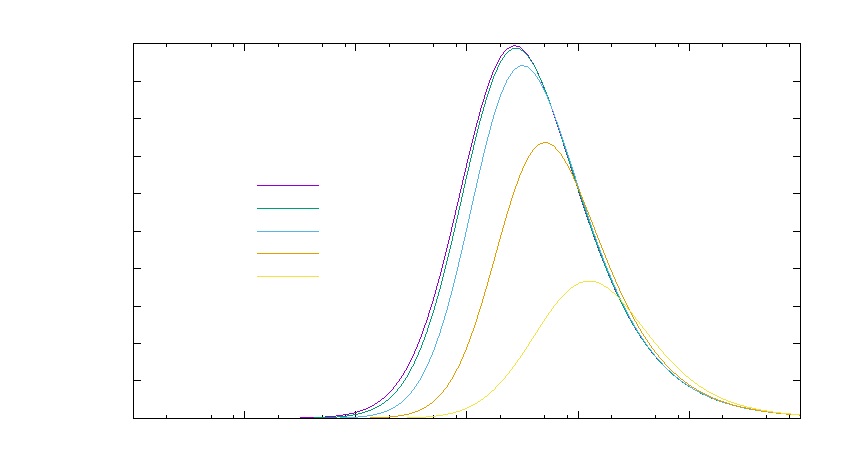
\includegraphics{img/dq1L}}%
    \gplfronttext
  \end{picture}%
\endgroup

\end{subfigure}\\%
\begin{subfigure}[t]{\textwidth}
	% GNUPLOT: LaTeX picture with Postscript
\begingroup
  \makeatletter
  \providecommand\color[2][]{%
    \GenericError{(gnuplot) \space\space\space\@spaces}{%
      Package color not loaded in conjunction with
      terminal option `colourtext'%
    }{See the gnuplot documentation for explanation.%
    }{Either use 'blacktext' in gnuplot or load the package
      color.sty in LaTeX.}%
    \renewcommand\color[2][]{}%
  }%
  \providecommand\includegraphics[2][]{%
    \GenericError{(gnuplot) \space\space\space\@spaces}{%
      Package graphicx or graphics not loaded%
    }{See the gnuplot documentation for explanation.%
    }{The gnuplot epslatex terminal needs graphicx.sty or graphics.sty.}%
    \renewcommand\includegraphics[2][]{}%
  }%
  \providecommand\rotatebox[2]{#2}%
  \@ifundefined{ifGPcolor}{%
    \newif\ifGPcolor
    \GPcolorfalse
  }{}%
  \@ifundefined{ifGPblacktext}{%
    \newif\ifGPblacktext
    \GPblacktexttrue
  }{}%
  % define a \g@addto@macro without @ in the name:
  \let\gplgaddtomacro\g@addto@macro
  % define empty templates for all commands taking text:
  \gdef\gplbacktext{}%
  \gdef\gplfronttext{}%
  \makeatother
  \ifGPblacktext
    % no textcolor at all
    \def\colorrgb#1{}%
    \def\colorgray#1{}%
  \else
    % gray or color?
    \ifGPcolor
      \def\colorrgb#1{\color[rgb]{#1}}%
      \def\colorgray#1{\color[gray]{#1}}%
      \expandafter\def\csname LTw\endcsname{\color{white}}%
      \expandafter\def\csname LTb\endcsname{\color{black}}%
      \expandafter\def\csname LTa\endcsname{\color{black}}%
      \expandafter\def\csname LT0\endcsname{\color[rgb]{1,0,0}}%
      \expandafter\def\csname LT1\endcsname{\color[rgb]{0,1,0}}%
      \expandafter\def\csname LT2\endcsname{\color[rgb]{0,0,1}}%
      \expandafter\def\csname LT3\endcsname{\color[rgb]{1,0,1}}%
      \expandafter\def\csname LT4\endcsname{\color[rgb]{0,1,1}}%
      \expandafter\def\csname LT5\endcsname{\color[rgb]{1,1,0}}%
      \expandafter\def\csname LT6\endcsname{\color[rgb]{0,0,0}}%
      \expandafter\def\csname LT7\endcsname{\color[rgb]{1,0.3,0}}%
      \expandafter\def\csname LT8\endcsname{\color[rgb]{0.5,0.5,0.5}}%
    \else
      % gray
      \def\colorrgb#1{\color{black}}%
      \def\colorgray#1{\color[gray]{#1}}%
      \expandafter\def\csname LTw\endcsname{\color{white}}%
      \expandafter\def\csname LTb\endcsname{\color{black}}%
      \expandafter\def\csname LTa\endcsname{\color{black}}%
      \expandafter\def\csname LT0\endcsname{\color{black}}%
      \expandafter\def\csname LT1\endcsname{\color{black}}%
      \expandafter\def\csname LT2\endcsname{\color{black}}%
      \expandafter\def\csname LT3\endcsname{\color{black}}%
      \expandafter\def\csname LT4\endcsname{\color{black}}%
      \expandafter\def\csname LT5\endcsname{\color{black}}%
      \expandafter\def\csname LT6\endcsname{\color{black}}%
      \expandafter\def\csname LT7\endcsname{\color{black}}%
      \expandafter\def\csname LT8\endcsname{\color{black}}%
    \fi
  \fi
    \setlength{\unitlength}{0.0500bp}%
    \ifx\gptboxheight\undefined%
      \newlength{\gptboxheight}%
      \newlength{\gptboxwidth}%
      \newsavebox{\gptboxtext}%
    \fi%
    \setlength{\fboxrule}{0.5pt}%
    \setlength{\fboxsep}{1pt}%
\begin{picture}(7920.00,4082.40)%
    \gplgaddtomacro\gplbacktext{%
      \csname LTb\endcsname%
      \put(990,220){\makebox(0,0)[r]{\strut{}-0.010}}%
      \put(990,670){\makebox(0,0)[r]{\strut{}-0.008}}%
      \put(990,1120){\makebox(0,0)[r]{\strut{}-0.006}}%
      \put(990,1569){\makebox(0,0)[r]{\strut{}-0.004}}%
      \put(990,2019){\makebox(0,0)[r]{\strut{}-0.002}}%
      \put(990,2469){\makebox(0,0)[r]{\strut{}0.000}}%
      \put(990,2919){\makebox(0,0)[r]{\strut{}0.002}}%
      \put(990,3368){\makebox(0,0)[r]{\strut{}0.004}}%
      \put(990,3818){\makebox(0,0)[r]{\strut{}0.006}}%
      \put(1122,0){\makebox(0,0){\strut{}$0.001$}}%
      \put(2189,0){\makebox(0,0){\strut{}$0.01$}}%
      \put(3255,0){\makebox(0,0){\strut{}$0.1$}}%
      \put(4322,0){\makebox(0,0){\strut{}$1$}}%
      \put(5389,0){\makebox(0,0){\strut{}$10$}}%
      \put(6455,0){\makebox(0,0){\strut{}$100$}}%
      \put(7522,0){\makebox(0,0){\strut{}$1000$}}%
      \put(1250,3458){\makebox(0,0)[l]{\strut{}(c) $d_{P,q}^{(1)}(\eta)$}}%
    }%
    \gplgaddtomacro\gplfronttext{%
      \csname LTb\endcsname%
      \put(1254,1273){\makebox(0,0)[l]{\strut{}$Q^2=10^{-2}$}}%
      \csname LTb\endcsname%
      \put(1254,1053){\makebox(0,0)[l]{\strut{}$Q^2=10^0$}}%
      \csname LTb\endcsname%
      \put(1254,833){\makebox(0,0)[l]{\strut{}$Q^2=10^1$}}%
      \csname LTb\endcsname%
      \put(1254,613){\makebox(0,0)[l]{\strut{}$Q^2=10^2$}}%
      \csname LTb\endcsname%
      \put(1254,393){\makebox(0,0)[l]{\strut{}$Q^2=10^3$}}%
    }%
    \gplbacktext
    \put(0,0){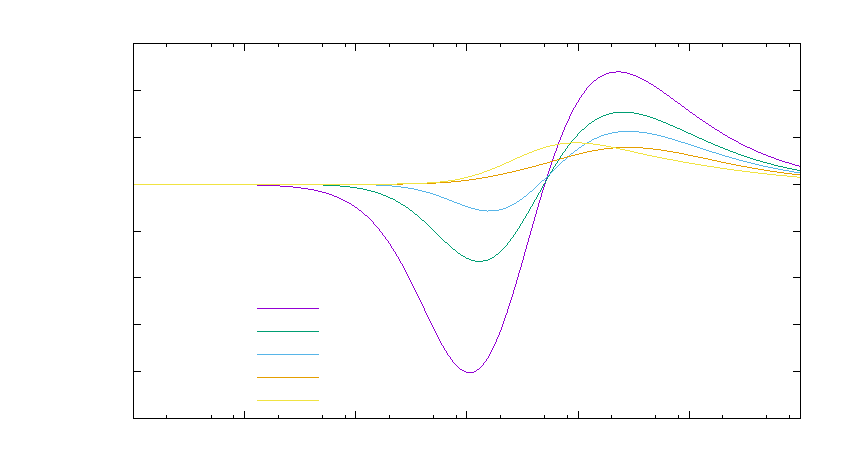
\includegraphics{img/dq1P}}%
    \gplfronttext
  \end{picture}%
\endgroup

\end{subfigure}
\caption{next-to-leading order scaling functions $d_{k,q}^{(1)}(\eta,\xi)$ plotted as function of $\eta=s/(4m^2)-1$ for different values of $Q^2$ in units of $\si{\GeV^2}$ at $m=\SI{4.75}{\GeV}$ (i.e. different values of $\xi=Q^2/m^2$) }\label{fig:dq1}
\end{figure}

\clearpage
\pagebreak
